\documentclass[11pt]{article}

    \usepackage[breakable]{tcolorbox}
    \usepackage{parskip} % Stop auto-indenting (to mimic markdown behaviour)
    

    % Basic figure setup, for now with no caption control since it's done
    % automatically by Pandoc (which extracts ![](path) syntax from Markdown).
    \usepackage{graphicx}
    % Maintain compatibility with old templates. Remove in nbconvert 6.0
    \let\Oldincludegraphics\includegraphics
    % Ensure that by default, figures have no caption (until we provide a
    % proper Figure object with a Caption API and a way to capture that
    % in the conversion process - todo).
    \usepackage{caption}
    \DeclareCaptionFormat{nocaption}{}
    \captionsetup{format=nocaption,aboveskip=0pt,belowskip=0pt}

    \usepackage{float}
    \floatplacement{figure}{H} % forces figures to be placed at the correct location
    \usepackage{xcolor} % Allow colors to be defined
    \usepackage{enumerate} % Needed for markdown enumerations to work
    \usepackage{geometry} % Used to adjust the document margins
    \usepackage{amsmath} % Equations
    \usepackage{amssymb} % Equations
    \usepackage{textcomp} % defines textquotesingle
    % Hack from http://tex.stackexchange.com/a/47451/13684:
    \AtBeginDocument{%
        \def\PYZsq{\textquotesingle}% Upright quotes in Pygmentized code
    }
    \usepackage{upquote} % Upright quotes for verbatim code
    \usepackage{eurosym} % defines \euro

    \usepackage{iftex}
    \ifPDFTeX
        \usepackage[T1]{fontenc}
        \IfFileExists{alphabeta.sty}{
              \usepackage{alphabeta}
          }{
              \usepackage[mathletters]{ucs}
              \usepackage[utf8x]{inputenc}
          }
    \else
        \usepackage{fontspec}
        \usepackage{unicode-math}
    \fi

    \usepackage{fancyvrb} % verbatim replacement that allows latex
    \usepackage{grffile} % extends the file name processing of package graphics
                         % to support a larger range
    \makeatletter % fix for old versions of grffile with XeLaTeX
    \@ifpackagelater{grffile}{2019/11/01}
    {
      % Do nothing on new versions
    }
    {
      \def\Gread@@xetex#1{%
        \IfFileExists{"\Gin@base".bb}%
        {\Gread@eps{\Gin@base.bb}}%
        {\Gread@@xetex@aux#1}%
      }
    }
    \makeatother
    \usepackage[Export]{adjustbox} % Used to constrain images to a maximum size
    \adjustboxset{max size={0.9\linewidth}{0.9\paperheight}}

    % The hyperref package gives us a pdf with properly built
    % internal navigation ('pdf bookmarks' for the table of contents,
    % internal cross-reference links, web links for URLs, etc.)
    \usepackage{hyperref}
    % The default LaTeX title has an obnoxious amount of whitespace. By default,
    % titling removes some of it. It also provides customization options.
    \usepackage{titling}
    \usepackage{longtable} % longtable support required by pandoc >1.10
    \usepackage{booktabs}  % table support for pandoc > 1.12.2
    \usepackage{array}     % table support for pandoc >= 2.11.3
    \usepackage{calc}      % table minipage width calculation for pandoc >= 2.11.1
    \usepackage[inline]{enumitem} % IRkernel/repr support (it uses the enumerate* environment)
    \usepackage[normalem]{ulem} % ulem is needed to support strikethroughs (\sout)
                                % normalem makes italics be italics, not underlines
    \usepackage{mathrsfs}
    

    
    % Colors for the hyperref package
    \definecolor{urlcolor}{rgb}{0,.145,.698}
    \definecolor{linkcolor}{rgb}{.71,0.21,0.01}
    \definecolor{citecolor}{rgb}{.12,.54,.11}

    % ANSI colors
    \definecolor{ansi-black}{HTML}{3E424D}
    \definecolor{ansi-black-intense}{HTML}{282C36}
    \definecolor{ansi-red}{HTML}{E75C58}
    \definecolor{ansi-red-intense}{HTML}{B22B31}
    \definecolor{ansi-green}{HTML}{00A250}
    \definecolor{ansi-green-intense}{HTML}{007427}
    \definecolor{ansi-yellow}{HTML}{DDB62B}
    \definecolor{ansi-yellow-intense}{HTML}{B27D12}
    \definecolor{ansi-blue}{HTML}{208FFB}
    \definecolor{ansi-blue-intense}{HTML}{0065CA}
    \definecolor{ansi-magenta}{HTML}{D160C4}
    \definecolor{ansi-magenta-intense}{HTML}{A03196}
    \definecolor{ansi-cyan}{HTML}{60C6C8}
    \definecolor{ansi-cyan-intense}{HTML}{258F8F}
    \definecolor{ansi-white}{HTML}{C5C1B4}
    \definecolor{ansi-white-intense}{HTML}{A1A6B2}
    \definecolor{ansi-default-inverse-fg}{HTML}{FFFFFF}
    \definecolor{ansi-default-inverse-bg}{HTML}{000000}

    % common color for the border for error outputs.
    \definecolor{outerrorbackground}{HTML}{FFDFDF}

    % commands and environments needed by pandoc snippets
    % extracted from the output of `pandoc -s`
    \providecommand{\tightlist}{%
      \setlength{\itemsep}{0pt}\setlength{\parskip}{0pt}}
    \DefineVerbatimEnvironment{Highlighting}{Verbatim}{commandchars=\\\{\}}
    % Add ',fontsize=\small' for more characters per line
    \newenvironment{Shaded}{}{}
    \newcommand{\KeywordTok}[1]{\textcolor[rgb]{0.00,0.44,0.13}{\textbf{{#1}}}}
    \newcommand{\DataTypeTok}[1]{\textcolor[rgb]{0.56,0.13,0.00}{{#1}}}
    \newcommand{\DecValTok}[1]{\textcolor[rgb]{0.25,0.63,0.44}{{#1}}}
    \newcommand{\BaseNTok}[1]{\textcolor[rgb]{0.25,0.63,0.44}{{#1}}}
    \newcommand{\FloatTok}[1]{\textcolor[rgb]{0.25,0.63,0.44}{{#1}}}
    \newcommand{\CharTok}[1]{\textcolor[rgb]{0.25,0.44,0.63}{{#1}}}
    \newcommand{\StringTok}[1]{\textcolor[rgb]{0.25,0.44,0.63}{{#1}}}
    \newcommand{\CommentTok}[1]{\textcolor[rgb]{0.38,0.63,0.69}{\textit{{#1}}}}
    \newcommand{\OtherTok}[1]{\textcolor[rgb]{0.00,0.44,0.13}{{#1}}}
    \newcommand{\AlertTok}[1]{\textcolor[rgb]{1.00,0.00,0.00}{\textbf{{#1}}}}
    \newcommand{\FunctionTok}[1]{\textcolor[rgb]{0.02,0.16,0.49}{{#1}}}
    \newcommand{\RegionMarkerTok}[1]{{#1}}
    \newcommand{\ErrorTok}[1]{\textcolor[rgb]{1.00,0.00,0.00}{\textbf{{#1}}}}
    \newcommand{\NormalTok}[1]{{#1}}

    % Additional commands for more recent versions of Pandoc
    \newcommand{\ConstantTok}[1]{\textcolor[rgb]{0.53,0.00,0.00}{{#1}}}
    \newcommand{\SpecialCharTok}[1]{\textcolor[rgb]{0.25,0.44,0.63}{{#1}}}
    \newcommand{\VerbatimStringTok}[1]{\textcolor[rgb]{0.25,0.44,0.63}{{#1}}}
    \newcommand{\SpecialStringTok}[1]{\textcolor[rgb]{0.73,0.40,0.53}{{#1}}}
    \newcommand{\ImportTok}[1]{{#1}}
    \newcommand{\DocumentationTok}[1]{\textcolor[rgb]{0.73,0.13,0.13}{\textit{{#1}}}}
    \newcommand{\AnnotationTok}[1]{\textcolor[rgb]{0.38,0.63,0.69}{\textbf{\textit{{#1}}}}}
    \newcommand{\CommentVarTok}[1]{\textcolor[rgb]{0.38,0.63,0.69}{\textbf{\textit{{#1}}}}}
    \newcommand{\VariableTok}[1]{\textcolor[rgb]{0.10,0.09,0.49}{{#1}}}
    \newcommand{\ControlFlowTok}[1]{\textcolor[rgb]{0.00,0.44,0.13}{\textbf{{#1}}}}
    \newcommand{\OperatorTok}[1]{\textcolor[rgb]{0.40,0.40,0.40}{{#1}}}
    \newcommand{\BuiltInTok}[1]{{#1}}
    \newcommand{\ExtensionTok}[1]{{#1}}
    \newcommand{\PreprocessorTok}[1]{\textcolor[rgb]{0.74,0.48,0.00}{{#1}}}
    \newcommand{\AttributeTok}[1]{\textcolor[rgb]{0.49,0.56,0.16}{{#1}}}
    \newcommand{\InformationTok}[1]{\textcolor[rgb]{0.38,0.63,0.69}{\textbf{\textit{{#1}}}}}
    \newcommand{\WarningTok}[1]{\textcolor[rgb]{0.38,0.63,0.69}{\textbf{\textit{{#1}}}}}


    % Define a nice break command that doesn't care if a line doesn't already
    % exist.
    \def\br{\hspace*{\fill} \\* }
    % Math Jax compatibility definitions
    \def\gt{>}
    \def\lt{<}
    \let\Oldtex\TeX
    \let\Oldlatex\LaTeX
    \renewcommand{\TeX}{\textrm{\Oldtex}}
    \renewcommand{\LaTeX}{\textrm{\Oldlatex}}
    % Document parameters
    % Document title
    \title{final}
    
    
    
    
    
% Pygments definitions
\makeatletter
\def\PY@reset{\let\PY@it=\relax \let\PY@bf=\relax%
    \let\PY@ul=\relax \let\PY@tc=\relax%
    \let\PY@bc=\relax \let\PY@ff=\relax}
\def\PY@tok#1{\csname PY@tok@#1\endcsname}
\def\PY@toks#1+{\ifx\relax#1\empty\else%
    \PY@tok{#1}\expandafter\PY@toks\fi}
\def\PY@do#1{\PY@bc{\PY@tc{\PY@ul{%
    \PY@it{\PY@bf{\PY@ff{#1}}}}}}}
\def\PY#1#2{\PY@reset\PY@toks#1+\relax+\PY@do{#2}}

\@namedef{PY@tok@w}{\def\PY@tc##1{\textcolor[rgb]{0.73,0.73,0.73}{##1}}}
\@namedef{PY@tok@c}{\let\PY@it=\textit\def\PY@tc##1{\textcolor[rgb]{0.24,0.48,0.48}{##1}}}
\@namedef{PY@tok@cp}{\def\PY@tc##1{\textcolor[rgb]{0.61,0.40,0.00}{##1}}}
\@namedef{PY@tok@k}{\let\PY@bf=\textbf\def\PY@tc##1{\textcolor[rgb]{0.00,0.50,0.00}{##1}}}
\@namedef{PY@tok@kp}{\def\PY@tc##1{\textcolor[rgb]{0.00,0.50,0.00}{##1}}}
\@namedef{PY@tok@kt}{\def\PY@tc##1{\textcolor[rgb]{0.69,0.00,0.25}{##1}}}
\@namedef{PY@tok@o}{\def\PY@tc##1{\textcolor[rgb]{0.40,0.40,0.40}{##1}}}
\@namedef{PY@tok@ow}{\let\PY@bf=\textbf\def\PY@tc##1{\textcolor[rgb]{0.67,0.13,1.00}{##1}}}
\@namedef{PY@tok@nb}{\def\PY@tc##1{\textcolor[rgb]{0.00,0.50,0.00}{##1}}}
\@namedef{PY@tok@nf}{\def\PY@tc##1{\textcolor[rgb]{0.00,0.00,1.00}{##1}}}
\@namedef{PY@tok@nc}{\let\PY@bf=\textbf\def\PY@tc##1{\textcolor[rgb]{0.00,0.00,1.00}{##1}}}
\@namedef{PY@tok@nn}{\let\PY@bf=\textbf\def\PY@tc##1{\textcolor[rgb]{0.00,0.00,1.00}{##1}}}
\@namedef{PY@tok@ne}{\let\PY@bf=\textbf\def\PY@tc##1{\textcolor[rgb]{0.80,0.25,0.22}{##1}}}
\@namedef{PY@tok@nv}{\def\PY@tc##1{\textcolor[rgb]{0.10,0.09,0.49}{##1}}}
\@namedef{PY@tok@no}{\def\PY@tc##1{\textcolor[rgb]{0.53,0.00,0.00}{##1}}}
\@namedef{PY@tok@nl}{\def\PY@tc##1{\textcolor[rgb]{0.46,0.46,0.00}{##1}}}
\@namedef{PY@tok@ni}{\let\PY@bf=\textbf\def\PY@tc##1{\textcolor[rgb]{0.44,0.44,0.44}{##1}}}
\@namedef{PY@tok@na}{\def\PY@tc##1{\textcolor[rgb]{0.41,0.47,0.13}{##1}}}
\@namedef{PY@tok@nt}{\let\PY@bf=\textbf\def\PY@tc##1{\textcolor[rgb]{0.00,0.50,0.00}{##1}}}
\@namedef{PY@tok@nd}{\def\PY@tc##1{\textcolor[rgb]{0.67,0.13,1.00}{##1}}}
\@namedef{PY@tok@s}{\def\PY@tc##1{\textcolor[rgb]{0.73,0.13,0.13}{##1}}}
\@namedef{PY@tok@sd}{\let\PY@it=\textit\def\PY@tc##1{\textcolor[rgb]{0.73,0.13,0.13}{##1}}}
\@namedef{PY@tok@si}{\let\PY@bf=\textbf\def\PY@tc##1{\textcolor[rgb]{0.64,0.35,0.47}{##1}}}
\@namedef{PY@tok@se}{\let\PY@bf=\textbf\def\PY@tc##1{\textcolor[rgb]{0.67,0.36,0.12}{##1}}}
\@namedef{PY@tok@sr}{\def\PY@tc##1{\textcolor[rgb]{0.64,0.35,0.47}{##1}}}
\@namedef{PY@tok@ss}{\def\PY@tc##1{\textcolor[rgb]{0.10,0.09,0.49}{##1}}}
\@namedef{PY@tok@sx}{\def\PY@tc##1{\textcolor[rgb]{0.00,0.50,0.00}{##1}}}
\@namedef{PY@tok@m}{\def\PY@tc##1{\textcolor[rgb]{0.40,0.40,0.40}{##1}}}
\@namedef{PY@tok@gh}{\let\PY@bf=\textbf\def\PY@tc##1{\textcolor[rgb]{0.00,0.00,0.50}{##1}}}
\@namedef{PY@tok@gu}{\let\PY@bf=\textbf\def\PY@tc##1{\textcolor[rgb]{0.50,0.00,0.50}{##1}}}
\@namedef{PY@tok@gd}{\def\PY@tc##1{\textcolor[rgb]{0.63,0.00,0.00}{##1}}}
\@namedef{PY@tok@gi}{\def\PY@tc##1{\textcolor[rgb]{0.00,0.52,0.00}{##1}}}
\@namedef{PY@tok@gr}{\def\PY@tc##1{\textcolor[rgb]{0.89,0.00,0.00}{##1}}}
\@namedef{PY@tok@ge}{\let\PY@it=\textit}
\@namedef{PY@tok@gs}{\let\PY@bf=\textbf}
\@namedef{PY@tok@gp}{\let\PY@bf=\textbf\def\PY@tc##1{\textcolor[rgb]{0.00,0.00,0.50}{##1}}}
\@namedef{PY@tok@go}{\def\PY@tc##1{\textcolor[rgb]{0.44,0.44,0.44}{##1}}}
\@namedef{PY@tok@gt}{\def\PY@tc##1{\textcolor[rgb]{0.00,0.27,0.87}{##1}}}
\@namedef{PY@tok@err}{\def\PY@bc##1{{\setlength{\fboxsep}{\string -\fboxrule}\fcolorbox[rgb]{1.00,0.00,0.00}{1,1,1}{\strut ##1}}}}
\@namedef{PY@tok@kc}{\let\PY@bf=\textbf\def\PY@tc##1{\textcolor[rgb]{0.00,0.50,0.00}{##1}}}
\@namedef{PY@tok@kd}{\let\PY@bf=\textbf\def\PY@tc##1{\textcolor[rgb]{0.00,0.50,0.00}{##1}}}
\@namedef{PY@tok@kn}{\let\PY@bf=\textbf\def\PY@tc##1{\textcolor[rgb]{0.00,0.50,0.00}{##1}}}
\@namedef{PY@tok@kr}{\let\PY@bf=\textbf\def\PY@tc##1{\textcolor[rgb]{0.00,0.50,0.00}{##1}}}
\@namedef{PY@tok@bp}{\def\PY@tc##1{\textcolor[rgb]{0.00,0.50,0.00}{##1}}}
\@namedef{PY@tok@fm}{\def\PY@tc##1{\textcolor[rgb]{0.00,0.00,1.00}{##1}}}
\@namedef{PY@tok@vc}{\def\PY@tc##1{\textcolor[rgb]{0.10,0.09,0.49}{##1}}}
\@namedef{PY@tok@vg}{\def\PY@tc##1{\textcolor[rgb]{0.10,0.09,0.49}{##1}}}
\@namedef{PY@tok@vi}{\def\PY@tc##1{\textcolor[rgb]{0.10,0.09,0.49}{##1}}}
\@namedef{PY@tok@vm}{\def\PY@tc##1{\textcolor[rgb]{0.10,0.09,0.49}{##1}}}
\@namedef{PY@tok@sa}{\def\PY@tc##1{\textcolor[rgb]{0.73,0.13,0.13}{##1}}}
\@namedef{PY@tok@sb}{\def\PY@tc##1{\textcolor[rgb]{0.73,0.13,0.13}{##1}}}
\@namedef{PY@tok@sc}{\def\PY@tc##1{\textcolor[rgb]{0.73,0.13,0.13}{##1}}}
\@namedef{PY@tok@dl}{\def\PY@tc##1{\textcolor[rgb]{0.73,0.13,0.13}{##1}}}
\@namedef{PY@tok@s2}{\def\PY@tc##1{\textcolor[rgb]{0.73,0.13,0.13}{##1}}}
\@namedef{PY@tok@sh}{\def\PY@tc##1{\textcolor[rgb]{0.73,0.13,0.13}{##1}}}
\@namedef{PY@tok@s1}{\def\PY@tc##1{\textcolor[rgb]{0.73,0.13,0.13}{##1}}}
\@namedef{PY@tok@mb}{\def\PY@tc##1{\textcolor[rgb]{0.40,0.40,0.40}{##1}}}
\@namedef{PY@tok@mf}{\def\PY@tc##1{\textcolor[rgb]{0.40,0.40,0.40}{##1}}}
\@namedef{PY@tok@mh}{\def\PY@tc##1{\textcolor[rgb]{0.40,0.40,0.40}{##1}}}
\@namedef{PY@tok@mi}{\def\PY@tc##1{\textcolor[rgb]{0.40,0.40,0.40}{##1}}}
\@namedef{PY@tok@il}{\def\PY@tc##1{\textcolor[rgb]{0.40,0.40,0.40}{##1}}}
\@namedef{PY@tok@mo}{\def\PY@tc##1{\textcolor[rgb]{0.40,0.40,0.40}{##1}}}
\@namedef{PY@tok@ch}{\let\PY@it=\textit\def\PY@tc##1{\textcolor[rgb]{0.24,0.48,0.48}{##1}}}
\@namedef{PY@tok@cm}{\let\PY@it=\textit\def\PY@tc##1{\textcolor[rgb]{0.24,0.48,0.48}{##1}}}
\@namedef{PY@tok@cpf}{\let\PY@it=\textit\def\PY@tc##1{\textcolor[rgb]{0.24,0.48,0.48}{##1}}}
\@namedef{PY@tok@c1}{\let\PY@it=\textit\def\PY@tc##1{\textcolor[rgb]{0.24,0.48,0.48}{##1}}}
\@namedef{PY@tok@cs}{\let\PY@it=\textit\def\PY@tc##1{\textcolor[rgb]{0.24,0.48,0.48}{##1}}}

\def\PYZbs{\char`\\}
\def\PYZus{\char`\_}
\def\PYZob{\char`\{}
\def\PYZcb{\char`\}}
\def\PYZca{\char`\^}
\def\PYZam{\char`\&}
\def\PYZlt{\char`\<}
\def\PYZgt{\char`\>}
\def\PYZsh{\char`\#}
\def\PYZpc{\char`\%}
\def\PYZdl{\char`\$}
\def\PYZhy{\char`\-}
\def\PYZsq{\char`\'}
\def\PYZdq{\char`\"}
\def\PYZti{\char`\~}
% for compatibility with earlier versions
\def\PYZat{@}
\def\PYZlb{[}
\def\PYZrb{]}
\makeatother


    % For linebreaks inside Verbatim environment from package fancyvrb.
    \makeatletter
        \newbox\Wrappedcontinuationbox
        \newbox\Wrappedvisiblespacebox
        \newcommand*\Wrappedvisiblespace {\textcolor{red}{\textvisiblespace}}
        \newcommand*\Wrappedcontinuationsymbol {\textcolor{red}{\llap{\tiny$\m@th\hookrightarrow$}}}
        \newcommand*\Wrappedcontinuationindent {3ex }
        \newcommand*\Wrappedafterbreak {\kern\Wrappedcontinuationindent\copy\Wrappedcontinuationbox}
        % Take advantage of the already applied Pygments mark-up to insert
        % potential linebreaks for TeX processing.
        %        {, <, #, %, $, ' and ": go to next line.
        %        _, }, ^, &, >, - and ~: stay at end of broken line.
        % Use of \textquotesingle for straight quote.
        \newcommand*\Wrappedbreaksatspecials {%
            \def\PYGZus{\discretionary{\char`\_}{\Wrappedafterbreak}{\char`\_}}%
            \def\PYGZob{\discretionary{}{\Wrappedafterbreak\char`\{}{\char`\{}}%
            \def\PYGZcb{\discretionary{\char`\}}{\Wrappedafterbreak}{\char`\}}}%
            \def\PYGZca{\discretionary{\char`\^}{\Wrappedafterbreak}{\char`\^}}%
            \def\PYGZam{\discretionary{\char`\&}{\Wrappedafterbreak}{\char`\&}}%
            \def\PYGZlt{\discretionary{}{\Wrappedafterbreak\char`\<}{\char`\<}}%
            \def\PYGZgt{\discretionary{\char`\>}{\Wrappedafterbreak}{\char`\>}}%
            \def\PYGZsh{\discretionary{}{\Wrappedafterbreak\char`\#}{\char`\#}}%
            \def\PYGZpc{\discretionary{}{\Wrappedafterbreak\char`\%}{\char`\%}}%
            \def\PYGZdl{\discretionary{}{\Wrappedafterbreak\char`\$}{\char`\$}}%
            \def\PYGZhy{\discretionary{\char`\-}{\Wrappedafterbreak}{\char`\-}}%
            \def\PYGZsq{\discretionary{}{\Wrappedafterbreak\textquotesingle}{\textquotesingle}}%
            \def\PYGZdq{\discretionary{}{\Wrappedafterbreak\char`\"}{\char`\"}}%
            \def\PYGZti{\discretionary{\char`\~}{\Wrappedafterbreak}{\char`\~}}%
        }
        % Some characters . , ; ? ! / are not pygmentized.
        % This macro makes them "active" and they will insert potential linebreaks
        \newcommand*\Wrappedbreaksatpunct {%
            \lccode`\~`\.\lowercase{\def~}{\discretionary{\hbox{\char`\.}}{\Wrappedafterbreak}{\hbox{\char`\.}}}%
            \lccode`\~`\,\lowercase{\def~}{\discretionary{\hbox{\char`\,}}{\Wrappedafterbreak}{\hbox{\char`\,}}}%
            \lccode`\~`\;\lowercase{\def~}{\discretionary{\hbox{\char`\;}}{\Wrappedafterbreak}{\hbox{\char`\;}}}%
            \lccode`\~`\:\lowercase{\def~}{\discretionary{\hbox{\char`\:}}{\Wrappedafterbreak}{\hbox{\char`\:}}}%
            \lccode`\~`\?\lowercase{\def~}{\discretionary{\hbox{\char`\?}}{\Wrappedafterbreak}{\hbox{\char`\?}}}%
            \lccode`\~`\!\lowercase{\def~}{\discretionary{\hbox{\char`\!}}{\Wrappedafterbreak}{\hbox{\char`\!}}}%
            \lccode`\~`\/\lowercase{\def~}{\discretionary{\hbox{\char`\/}}{\Wrappedafterbreak}{\hbox{\char`\/}}}%
            \catcode`\.\active
            \catcode`\,\active
            \catcode`\;\active
            \catcode`\:\active
            \catcode`\?\active
            \catcode`\!\active
            \catcode`\/\active
            \lccode`\~`\~
        }
    \makeatother

    \let\OriginalVerbatim=\Verbatim
    \makeatletter
    \renewcommand{\Verbatim}[1][1]{%
        %\parskip\z@skip
        \sbox\Wrappedcontinuationbox {\Wrappedcontinuationsymbol}%
        \sbox\Wrappedvisiblespacebox {\FV@SetupFont\Wrappedvisiblespace}%
        \def\FancyVerbFormatLine ##1{\hsize\linewidth
            \vtop{\raggedright\hyphenpenalty\z@\exhyphenpenalty\z@
                \doublehyphendemerits\z@\finalhyphendemerits\z@
                \strut ##1\strut}%
        }%
        % If the linebreak is at a space, the latter will be displayed as visible
        % space at end of first line, and a continuation symbol starts next line.
        % Stretch/shrink are however usually zero for typewriter font.
        \def\FV@Space {%
            \nobreak\hskip\z@ plus\fontdimen3\font minus\fontdimen4\font
            \discretionary{\copy\Wrappedvisiblespacebox}{\Wrappedafterbreak}
            {\kern\fontdimen2\font}%
        }%

        % Allow breaks at special characters using \PYG... macros.
        \Wrappedbreaksatspecials
        % Breaks at punctuation characters . , ; ? ! and / need catcode=\active
        \OriginalVerbatim[#1,codes*=\Wrappedbreaksatpunct]%
    }
    \makeatother

    % Exact colors from NB
    \definecolor{incolor}{HTML}{303F9F}
    \definecolor{outcolor}{HTML}{D84315}
    \definecolor{cellborder}{HTML}{CFCFCF}
    \definecolor{cellbackground}{HTML}{F7F7F7}

    % prompt
    \makeatletter
    \newcommand{\boxspacing}{\kern\kvtcb@left@rule\kern\kvtcb@boxsep}
    \makeatother
    \newcommand{\prompt}[4]{
        {\ttfamily\llap{{\color{#2}[#3]:\hspace{3pt}#4}}\vspace{-\baselineskip}}
    }
    

    
    % Prevent overflowing lines due to hard-to-break entities
    \sloppy
    % Setup hyperref package
    \hypersetup{
      breaklinks=true,  % so long urls are correctly broken across lines
      colorlinks=true,
      urlcolor=urlcolor,
      linkcolor=linkcolor,
      citecolor=citecolor,
      }
    % Slightly bigger margins than the latex defaults
    
    \geometry{verbose,tmargin=1in,bmargin=1in,lmargin=1in,rmargin=1in}
    
    

\begin{document}
    
    \maketitle
    
    

    
    \hypertarget{convex-optimization---homework-3}{%
\section{Convex Optimization - Homework
3}\label{convex-optimization---homework-3}}

Report plots, comments and theoretical results in a pdf file. Send your
code together with the requested functions and a main script reproducing
all your experiments. You can use Matlab, Python or Julia.

Given \(x_1,...,x_n \in \mathbb{R}^d\) data vectors and
\(y_1,...,y_n \in \mathbb{R}\) observations, we are searching for
regression parameters \(w \in \mathbb{R}^d\) which fit data inputs to
observations \(y\) by minimizing their squared difference. In a high
dimensional setting (when \(n \ll d\)) a \(\ell_1\) norm penalty is
often used on the regression coefficients \(w\) in order to enforce
sparsity of the solution (so that \(w\) will only have a few non-zeros
entries). Such penalization has well known statistical properties, and
makes the model both more interpretable, and faster at test time.

From an optimization point of view we want to solve the following
problem called LASSO (which stands for Least Absolute Shrinkage Operator
and Selection Operator)

\begin{equation}
\tag{LASSO}
\begin{array}{ll}
\text{minimize} & \frac{1}{2} \left\lVert Xw - y \right\rVert^2_2 + \lambda \left\lVert w \right\rVert_1
\end{array}
\end{equation}

in the variable \(w \in \mathbb{R}^d\), where
\(X = (x^T_1, \ldots, x^T_n) \in \mathbb{R}^{n\times d},\, y = (y_1, \ldots, y_n) \in \mathbb{R}^n\)
and \(\lambda > 0\) is a regularization parameter.

    1. Derive the dual problem of LASSO and format it as a general Quadratic
Problem as follows

\begin{equation}
\tag{QP}
\begin{array}{ll}
\text{minimize} & v^TQv + p^Tv \\
\text{subject to} & Av \preceq b
\end{array}
\end{equation}

in variable \(v\in \mathbb{R}^n\), where \(Q \succeq 0\).

    We can repose the LASSO problem as the following problem

\begin{equation}
\tag{LASSO'}
\begin{array}{ll}
\displaystyle \min_{w \in \mathbb{R}^d,\, z \in \mathbb{R}^n} & \frac{1}{2} \left\lVert z \right\rVert^2_2 + \lambda \left\lVert w \right\rVert_1 \\
\text{subject to} & z = Xw - y 
\end{array}
\end{equation}

The associated Lagragian is

\begin{align*}
\mathcal{L}(w, z, v) &= \frac{1}{2} z^T z + \lambda \left\lVert w \right\rVert_1 - v^T (y-Xw+z)
\end{align*}

We can then calculate the dual function

\begin{align*}
g(v) &= \inf_{w, z} \frac{1}{2} z^T z + \lambda \left\lVert w \right\rVert_1 - v^T (y-Xw+z) \\
&= - v^T y + \inf_z \{ \frac{1}{2} z^T z - v^T z\} + \lambda \inf_w \{\left\lVert w \right\rVert_1 + \frac{1}{\lambda} v^T X w\} \\
&= \left\{ \begin{array}{ll} - v^T y - \frac{1}{2} v^T v & \text{if } \left\lVert X^T v \right\lVert_{\infty} \le \lambda \\
- \infty & \text{otherwise} \end{array}\right.
\end{align*}

We can obtain the dual problem

\begin{equation}
\tag{LASSO*}
\begin{array}{ll}
\text{maximize} & - v^T y - \frac{1}{2} v^T v \\
\text{subject to} & \left\lVert X^T v \right\lVert_{\infty} \le \lambda \\
\end{array}
\end{equation}

which can be simplified as follows

\begin{equation}
\tag{LASSO*}
\begin{array}{ll}
\displaystyle \min_{v \in \mathbb{R}^n} & \frac{1}{2} v^T v  + y^T v \\
\text{subject to} & - X^T v \le \lambda \cdot \mathbb{1}_d \\
& X^T v \le \lambda \cdot \mathbb{1}_d
\end{array}
\end{equation}

Finally, we can rewrite it as

\begin{equation}
\tag{QP}
\begin{array}{ll}
\text{minimize} & v^TQv + p^Tv \\
\text{subject to} & Av \preceq b
\end{array}
\end{equation}

with

\begin{itemize}
\tightlist
\item
  \(Q = \frac{1}{2} I_n \in \mathbb{R}^{n \times n}\), we have
  \(Q \succeq 0\).
\item
  \(p = y \in \mathbb{R}^{n}\)
\item
  \(b = \lambda \cdot \mathbb{1}_{2d} \in \mathbb{R}^{2d}\)
\end{itemize}

and \begin{equation*}
A = \left(
    \begin{array}{c}
    X^T \\
    -X^T
    \end{array}
\right)
\in \mathbb{R}^{2d \times n}
\end{equation*}

For the next question, we pose \(m=2d\).

    1. Impliment the barrier method to solve QP.

\begin{itemize}
\tightlist
\item
  Write a function
  \texttt{v\_seq\ =\ centering\_step(Q,\ p,\ A,\ b,\ t,\ v0,\ eps)}
  which impliments the Newton method to solve the centering step given
  the inputs \((Q, p, A, b)\), the barrier method parameter \(t\) (see
  lectures), initial variable \(v_0\) and a target precision
  \(\epsilon\). The function outputs the sequence of variables iterates
  \((v_i)_{i=1, \ldots, n_{\epsilon}}\), where \(n_{\epsilon}\) is the
  number of iterations to obtain the \(\epsilon\) precision. Use a
  backtracking line search with appropriate parameters.
\item
  Write a function
  \texttt{v\_seq\ =\ barr\_method(Q,\ p,\ A,\ b,\ v0,\ eps)} which
  implements the barrier method to solve QP using precedent function
  given the data inputs \((Q, p, A, b)\), a feasible point \(v_0\), a
  precision criterion \(\epsilon\). The function ouptuts the sequence of
  variables iterates \((v_i)_{i=1, \ldots, n_{\epsilon}}\), where
  \(n_{\epsilon}\) is the number of iterations to obtain the
  \(\epsilon\) precision.
\item
  Test your function on randomly generated matrices \(X\) and
  observations \(y\) withz \(\lambda = 10\). Plot precision criterion
  and gap \(f(v_t) - f^*\) in semilog scale (using the best value found
  for \(f\) as a surrogate for \(f^*\)). Repeat for different values of
  the barrier method parameter \(\mu = 2, 15, 50, 100, \ldots\) and
  check the impact on \(w\). What would be an appropriate choice for
  \(\mu\) ?
\end{itemize}

    We can write

\[
A = \left(\begin{array}{ccc}
& a_1^T & \\
\hline
& \vdots & \\
\hline
& a_m^T &
\end{array}\right)
\] with \(a_i \in \mathbb{R}^n\).

The barrier problem can be written as

\begin{equation}
\tag{Barrier}

\begin{array}{ll}
\displaystyle \min_{v \in \mathbb{R}^n} & t (v^T Q v + p^T v) + \phi(v) \\
\text{subject to} & \forall i \in [1, \cdots, m], \; a_i^T v - b_i \le 0
\end{array}

\end{equation}

We pose
\(\forall i \in [1, \cdots, m], \; f_i(v) = a_i^T v - b_i \in \mathbb{R}\).
With this notation,
\(\phi(v) = - \displaystyle \sum_{i=1}^m \log(-f_i(v))\).

From there, we can look at

\begin{align*}
\nabla \phi(v) &= \sum_{i=1}^m \frac{1}{- f_i(v)} \nabla f_i(v) \\
&= \sum_{i=1}^m \frac{1}{b_i - a_i^T v} a_i
\end{align*}

and

\begin{align*}
\nabla^2 \phi(v) &= \sum_{i=1}^m \frac{1}{f_i(v)^2} \nabla f_i(v) \nabla f_i(v)^T \\
&= \sum_{i=1}^m \frac{1}{(b_i - a_i^T v)^2} a_i a_i^T
\end{align*}

since \(\nabla^2 f_i(v) = 0\).

Lastly, to get \(w^*\) from the dual problem, we can use the fact that
the Lagragian is minimized by the optimal point, the gradient of the
Lagragian with respoect to \(z\) vanishes. Which gives us:

\begin{align*}
    \nabla_z \mathcal{L}(w^*, z^*, v^*) &= 0 \\
    &= z^* - v^* \\
    &= X w^* - y - v^*
\end{align*}

Given \(v^*, X\) and \(y\), we can get \(w^*\) by resolving the least
squares :

\begin{align*}
    w^* = X^{\dagger}(y + v^*)
\end{align*}

    \hypertarget{code-for-the-testing}{%
\subsection{Code for the testing}\label{code-for-the-testing}}

I decided to use Python to implement the testing on the data.

The following code only a part of the total code I wrote to do this, I
only kept the essential for readibility reasons. You can find the
complete code on this GitHub repository:
\url{https://github.com/gwatkinson/HW3}.

    \hypertarget{rapid-implementation}{%
\subsection{Rapid implementation}\label{rapid-implementation}}

In this section, I implemented the mentioned function quite fast, and
tested it on generated data.

    \begin{tcolorbox}[breakable, size=fbox, boxrule=1pt, pad at break*=1mm,colback=cellbackground, colframe=cellborder]
\prompt{In}{incolor}{183}{\boxspacing}
\begin{Verbatim}[commandchars=\\\{\}]
\PY{k+kn}{import} \PY{n+nn}{numpy} \PY{k}{as} \PY{n+nn}{np}

\PY{k+kn}{from} \PY{n+nn}{typing} \PY{k+kn}{import} \PY{n}{Callable}

\PY{n}{f\PYZus{}type} \PY{o}{=} \PY{n}{Callable}\PY{p}{[}\PY{p}{[}\PY{n}{np}\PY{o}{.}\PY{n}{array}\PY{p}{]}\PY{p}{,} \PY{n+nb}{float}\PY{p}{]}
\end{Verbatim}
\end{tcolorbox}

    \hypertarget{defining-the-functions}{%
\subsubsection{Defining the functions}\label{defining-the-functions}}

This cell defines the function of the problem, given the necessary
matrices.

    \begin{tcolorbox}[breakable, size=fbox, boxrule=1pt, pad at break*=1mm,colback=cellbackground, colframe=cellborder]
\prompt{In}{incolor}{194}{\boxspacing}
\begin{Verbatim}[commandchars=\\\{\}]
\PY{k}{def} \PY{n+nf}{f}\PY{p}{(}\PY{n}{v}\PY{p}{,} \PY{n}{Q}\PY{p}{,} \PY{n}{p}\PY{p}{)}\PY{p}{:}
    \PY{l+s+sd}{\PYZdq{}\PYZdq{}\PYZdq{}The original objective function f\PYZus{}0.\PYZdq{}\PYZdq{}\PYZdq{}}
    \PY{k}{return} \PY{n}{v}\PY{o}{.}\PY{n}{T} \PY{o}{@} \PY{n}{Q} \PY{o}{@} \PY{n}{v} \PY{o}{+} \PY{n}{p}\PY{o}{.}\PY{n}{T} \PY{o}{@} \PY{n}{v}

\PY{k}{def} \PY{n+nf}{grad\PYZus{}f}\PY{p}{(}\PY{n}{v}\PY{p}{,} \PY{n}{Q}\PY{p}{,} \PY{n}{p}\PY{p}{)}\PY{p}{:}
    \PY{l+s+sd}{\PYZdq{}\PYZdq{}\PYZdq{}The gradient of f.\PYZdq{}\PYZdq{}\PYZdq{}}
    \PY{k}{return} \PY{l+m+mi}{2} \PY{o}{*} \PY{n}{Q} \PY{o}{@} \PY{n}{v} \PY{o}{+} \PY{n}{p}


\PY{k}{def} \PY{n+nf}{hess\PYZus{}f}\PY{p}{(}\PY{n}{v}\PY{p}{,} \PY{n}{Q}\PY{p}{,} \PY{n}{p}\PY{p}{)}\PY{p}{:}
    \PY{l+s+sd}{\PYZdq{}\PYZdq{}\PYZdq{}The hessian of f.\PYZdq{}\PYZdq{}\PYZdq{}}
    \PY{k}{return} \PY{l+m+mi}{2} \PY{o}{*} \PY{n}{Q}


\PY{k}{def} \PY{n+nf}{g}\PY{p}{(}\PY{n}{v}\PY{p}{,} \PY{n}{A}\PY{p}{,} \PY{n}{b}\PY{p}{,} \PY{n}{i}\PY{p}{)}\PY{p}{:}
    \PY{l+s+sd}{\PYZdq{}\PYZdq{}\PYZdq{}The log affine constraints f\PYZus{}i.\PYZdq{}\PYZdq{}\PYZdq{}}
    \PY{n}{ai} \PY{o}{=} \PY{n}{A}\PY{p}{[}\PY{n}{i}\PY{p}{,} \PY{p}{:}\PY{p}{]}
    \PY{n}{bi} \PY{o}{=} \PY{n}{b}\PY{p}{[}\PY{n}{i}\PY{p}{]}
    \PY{k}{return} \PY{n+nb}{float}\PY{p}{(}\PY{n}{np}\PY{o}{.}\PY{n}{nan\PYZus{}to\PYZus{}num}\PY{p}{(}\PY{o}{\PYZhy{}}\PY{n}{np}\PY{o}{.}\PY{n}{log}\PY{p}{(}\PY{n}{bi} \PY{o}{\PYZhy{}} \PY{n}{ai}\PY{o}{.}\PY{n}{T} \PY{o}{@} \PY{n}{v}\PY{p}{)}\PY{p}{,} \PY{n}{nan}\PY{o}{=}\PY{n}{np}\PY{o}{.}\PY{n}{inf}\PY{p}{)}\PY{p}{)}

\PY{k}{def} \PY{n+nf}{grad\PYZus{}g}\PY{p}{(}\PY{n}{v}\PY{p}{,} \PY{n}{A}\PY{p}{,} \PY{n}{b}\PY{p}{,} \PY{n}{i}\PY{p}{)}\PY{p}{:}
    \PY{l+s+sd}{\PYZdq{}\PYZdq{}\PYZdq{}The gradient of the log affine constraints f\PYZus{}i.\PYZdq{}\PYZdq{}\PYZdq{}}
    \PY{n}{ai} \PY{o}{=} \PY{n}{A}\PY{p}{[}\PY{n}{i}\PY{p}{,} \PY{p}{:}\PY{p}{]}
    \PY{n}{bi} \PY{o}{=} \PY{n}{b}\PY{p}{[}\PY{n}{i}\PY{p}{]}
    \PY{k}{return} \PY{n}{ai} \PY{o}{/} \PY{p}{(}\PY{n}{bi} \PY{o}{\PYZhy{}} \PY{n}{ai}\PY{o}{.}\PY{n}{T} \PY{o}{@} \PY{n}{v}\PY{p}{)}

\PY{k}{def} \PY{n+nf}{hess\PYZus{}g}\PY{p}{(}\PY{n}{v}\PY{p}{,} \PY{n}{A}\PY{p}{,} \PY{n}{b}\PY{p}{,} \PY{n}{i}\PY{p}{)}\PY{p}{:}
    \PY{l+s+sd}{\PYZdq{}\PYZdq{}\PYZdq{}The hessian of the log affine constraints f\PYZus{}i.\PYZdq{}\PYZdq{}\PYZdq{}}
    \PY{n}{ai} \PY{o}{=} \PY{n}{A}\PY{p}{[}\PY{n}{i}\PY{p}{,} \PY{p}{:}\PY{p}{]}
    \PY{n}{bi} \PY{o}{=} \PY{n}{b}\PY{p}{[}\PY{n}{i}\PY{p}{]}
    \PY{k}{return} \PY{n}{ai}\PY{o}{.}\PY{n}{reshape}\PY{p}{(}\PY{o}{\PYZhy{}}\PY{l+m+mi}{1}\PY{p}{,} \PY{l+m+mi}{1}\PY{p}{)} \PY{o}{@} \PY{n}{ai}\PY{o}{.}\PY{n}{reshape}\PY{p}{(}\PY{o}{\PYZhy{}}\PY{l+m+mi}{1}\PY{p}{,} \PY{l+m+mi}{1}\PY{p}{)}\PY{o}{.}\PY{n}{T} \PY{o}{/} \PY{p}{(}\PY{n}{bi} \PY{o}{\PYZhy{}} \PY{n}{ai}\PY{o}{.}\PY{n}{T} \PY{o}{@} \PY{n}{v}\PY{p}{)} \PY{o}{*}\PY{o}{*} \PY{l+m+mi}{2}


\PY{k}{def} \PY{n+nf}{phi}\PY{p}{(}\PY{n}{v}\PY{p}{,} \PY{n}{A}\PY{p}{,} \PY{n}{b}\PY{p}{)}\PY{p}{:}
    \PY{l+s+sd}{\PYZdq{}\PYZdq{}\PYZdq{}The log barrier function phi.\PYZdq{}\PYZdq{}\PYZdq{}}
    \PY{n}{m} \PY{o}{=} \PY{n+nb}{len}\PY{p}{(}\PY{n}{b}\PY{p}{)}
    \PY{k}{return} \PY{n}{np}\PY{o}{.}\PY{n}{sum}\PY{p}{(}\PY{p}{[}\PY{n}{g}\PY{p}{(}\PY{n}{v}\PY{p}{,} \PY{n}{A}\PY{p}{,} \PY{n}{b}\PY{p}{,} \PY{n}{i}\PY{p}{)} \PY{k}{for} \PY{n}{i} \PY{o+ow}{in} \PY{n+nb}{range}\PY{p}{(}\PY{n}{m}\PY{p}{)}\PY{p}{]}\PY{p}{)}


\PY{k}{def} \PY{n+nf}{grad\PYZus{}phi}\PY{p}{(}\PY{n}{v}\PY{p}{,} \PY{n}{A}\PY{p}{,} \PY{n}{b}\PY{p}{)}\PY{p}{:}
    \PY{l+s+sd}{\PYZdq{}\PYZdq{}\PYZdq{}The gradient of the log barrier function.\PYZdq{}\PYZdq{}\PYZdq{}}
    \PY{n}{m} \PY{o}{=} \PY{n+nb}{len}\PY{p}{(}\PY{n}{b}\PY{p}{)}
    \PY{k}{return} \PY{n}{np}\PY{o}{.}\PY{n}{sum}\PY{p}{(}\PY{n}{np}\PY{o}{.}\PY{n}{array}\PY{p}{(}\PY{p}{[}\PY{n}{grad\PYZus{}g}\PY{p}{(}\PY{n}{v}\PY{p}{,} \PY{n}{A}\PY{p}{,} \PY{n}{b}\PY{p}{,} \PY{n}{i}\PY{p}{)} \PY{k}{for} \PY{n}{i} \PY{o+ow}{in} \PY{n+nb}{range}\PY{p}{(}\PY{n}{m}\PY{p}{)}\PY{p}{]}\PY{p}{)}\PY{p}{,} \PY{n}{axis}\PY{o}{=}\PY{l+m+mi}{0}\PY{p}{)}


\PY{k}{def} \PY{n+nf}{hess\PYZus{}phi}\PY{p}{(}\PY{n}{v}\PY{p}{,} \PY{n}{A}\PY{p}{,} \PY{n}{b}\PY{p}{)}\PY{p}{:}
    \PY{l+s+sd}{\PYZdq{}\PYZdq{}\PYZdq{}The hessian of the log barrier function.\PYZdq{}\PYZdq{}\PYZdq{}}
    \PY{n}{m} \PY{o}{=} \PY{n+nb}{len}\PY{p}{(}\PY{n}{b}\PY{p}{)}
    \PY{k}{return} \PY{n}{np}\PY{o}{.}\PY{n}{sum}\PY{p}{(}\PY{n}{np}\PY{o}{.}\PY{n}{array}\PY{p}{(}\PY{p}{[}\PY{n}{hess\PYZus{}g}\PY{p}{(}\PY{n}{v}\PY{p}{,} \PY{n}{A}\PY{p}{,} \PY{n}{b}\PY{p}{,} \PY{n}{i}\PY{p}{)} \PY{k}{for} \PY{n}{i} \PY{o+ow}{in} \PY{n+nb}{range}\PY{p}{(}\PY{n}{m}\PY{p}{)}\PY{p}{]}\PY{p}{)}\PY{p}{,} \PY{n}{axis}\PY{o}{=}\PY{l+m+mi}{0}\PY{p}{)}

\PY{k}{def} \PY{n+nf}{dual\PYZus{}func}\PY{p}{(}\PY{n}{v}\PY{p}{,} \PY{n}{y}\PY{p}{)}\PY{p}{:}
    \PY{l+s+sd}{\PYZdq{}\PYZdq{}\PYZdq{}The dual function (the inf of the Lagragian).\PYZdq{}\PYZdq{}\PYZdq{}}
    \PY{k}{return} \PY{o}{\PYZhy{}} \PY{l+m+mf}{0.5} \PY{o}{*} \PY{n}{v}\PY{o}{.}\PY{n}{T} \PY{o}{@} \PY{n}{v} \PY{o}{\PYZhy{}} \PY{n}{v}\PY{o}{.}\PY{n}{T} \PY{o}{@} \PY{n}{y}

\PY{k}{def} \PY{n+nf}{lasso\PYZus{}func}\PY{p}{(}\PY{n}{w}\PY{p}{,} \PY{n}{X}\PY{p}{,} \PY{n}{y}\PY{p}{,} \PY{n}{ld}\PY{p}{)}\PY{p}{:}
    \PY{l+s+sd}{\PYZdq{}\PYZdq{}\PYZdq{}The lasso function.\PYZdq{}\PYZdq{}\PYZdq{}}
    \PY{k}{return} \PY{l+m+mf}{0.5} \PY{o}{*} \PY{n}{np}\PY{o}{.}\PY{n}{linalg}\PY{o}{.}\PY{n}{norm}\PY{p}{(}\PY{n}{X} \PY{o}{@} \PY{n}{w} \PY{o}{\PYZhy{}} \PY{n}{y}\PY{p}{)}\PY{o}{*}\PY{o}{*}\PY{l+m+mi}{2} \PY{o}{+} \PY{n}{ld} \PY{o}{*} \PY{n}{np}\PY{o}{.}\PY{n}{linalg}\PY{o}{.}\PY{n}{norm}\PY{p}{(}\PY{n}{w}\PY{p}{,} \PY{l+m+mi}{1}\PY{p}{)}

\PY{k}{def} \PY{n+nf}{get\PYZus{}w\PYZus{}star}\PY{p}{(}\PY{n}{v\PYZus{}star}\PY{p}{,} \PY{n}{X}\PY{p}{,} \PY{n}{y}\PY{p}{)}\PY{p}{:}
    \PY{k}{return} \PY{n}{np}\PY{o}{.}\PY{n}{linalg}\PY{o}{.}\PY{n}{lstsq}\PY{p}{(}\PY{n}{X}\PY{p}{,} \PY{n}{y} \PY{o}{+} \PY{n}{v\PYZus{}star}\PY{p}{,} \PY{n}{rcond}\PY{o}{=}\PY{k+kc}{None}\PY{p}{)}\PY{p}{[}\PY{l+m+mi}{0}\PY{p}{]}
\end{Verbatim}
\end{tcolorbox}

    \hypertarget{algorithms}{%
\subsubsection{Algorithms}\label{algorithms}}

This cell implements the algorithms used for resolving the convex
problem.

We first define the \texttt{backtracking\_line\_search} abd the
\texttt{newton\_method} that works on any function, given the gradient
and hessian.

Then, the \texttt{centering\_step}, just applies the newton method to
the constrained quadratic problem.

Lastly, the \texttt{barr\_method} implements the barrier method for a
given \(\mu\).

    \begin{tcolorbox}[breakable, size=fbox, boxrule=1pt, pad at break*=1mm,colback=cellbackground, colframe=cellborder]
\prompt{In}{incolor}{195}{\boxspacing}
\begin{Verbatim}[commandchars=\\\{\}]
\PY{k}{def} \PY{n+nf}{newton\PYZus{}step}\PY{p}{(}\PY{n}{x}\PY{p}{:} \PY{n}{np}\PY{o}{.}\PY{n}{array}\PY{p}{,} \PY{n}{grad\PYZus{}f}\PY{p}{:} \PY{n}{f\PYZus{}type}\PY{p}{,} \PY{n}{hess\PYZus{}f}\PY{p}{:} \PY{n}{f\PYZus{}type}\PY{p}{)} \PY{o}{\PYZhy{}}\PY{o}{\PYZgt{}} \PY{n}{np}\PY{o}{.}\PY{n}{array}\PY{p}{:}
    \PY{n}{step} \PY{o}{=} \PY{o}{\PYZhy{}}\PY{n}{np}\PY{o}{.}\PY{n}{linalg}\PY{o}{.}\PY{n}{inv}\PY{p}{(}\PY{n}{hess\PYZus{}f}\PY{p}{(}\PY{n}{x}\PY{p}{)}\PY{p}{)} \PY{o}{@} \PY{n}{grad\PYZus{}f}\PY{p}{(}\PY{n}{x}\PY{p}{)}
    \PY{k}{return} \PY{n}{step}

\PY{k}{def} \PY{n+nf}{newton\PYZus{}decrement}\PY{p}{(}\PY{n}{x}\PY{p}{:} \PY{n}{np}\PY{o}{.}\PY{n}{array}\PY{p}{,} \PY{n}{grad\PYZus{}f}\PY{p}{:} \PY{n}{f\PYZus{}type}\PY{p}{,} \PY{n}{hess\PYZus{}f}\PY{p}{:} \PY{n}{f\PYZus{}type}\PY{p}{)} \PY{o}{\PYZhy{}}\PY{o}{\PYZgt{}} \PY{n+nb}{float}\PY{p}{:}
    \PY{n}{decrement} \PY{o}{=} \PY{n}{np}\PY{o}{.}\PY{n}{sqrt}\PY{p}{(}\PY{n}{grad\PYZus{}f}\PY{p}{(}\PY{n}{x}\PY{p}{)}\PY{o}{.}\PY{n}{transpose}\PY{p}{(}\PY{p}{)} \PY{o}{@} \PY{n}{np}\PY{o}{.}\PY{n}{linalg}\PY{o}{.}\PY{n}{inv}\PY{p}{(}\PY{n}{hess\PYZus{}f}\PY{p}{(}\PY{n}{x}\PY{p}{)}\PY{p}{)} \PY{o}{@} \PY{n}{grad\PYZus{}f}\PY{p}{(}\PY{n}{x}\PY{p}{)}\PY{p}{)}
    \PY{k}{return} \PY{n}{decrement}


\PY{k}{def} \PY{n+nf}{backtracking\PYZus{}line\PYZus{}search}\PY{p}{(}
    \PY{n}{x}\PY{p}{:} \PY{n}{np}\PY{o}{.}\PY{n}{array}\PY{p}{,} \PY{n}{f}\PY{p}{:} \PY{n}{f\PYZus{}type}\PY{p}{,} \PY{n}{grad\PYZus{}f}\PY{p}{:} \PY{n}{f\PYZus{}type}\PY{p}{,} \PY{n}{delta\PYZus{}x}\PY{p}{:} \PY{n}{np}\PY{o}{.}\PY{n}{array}\PY{p}{,}
    \PY{n}{alpha}\PY{p}{:} \PY{n+nb}{float}\PY{p}{,} \PY{n}{beta}\PY{p}{:} \PY{n+nb}{float}\PY{p}{,} \PY{n}{verbose}\PY{p}{:} \PY{n+nb}{bool} \PY{o}{=} \PY{k+kc}{False}
\PY{p}{)} \PY{o}{\PYZhy{}}\PY{o}{\PYZgt{}} \PY{n+nb}{float}\PY{p}{:}
    \PY{k}{assert} \PY{n}{alpha} \PY{o}{\PYZgt{}} \PY{l+m+mi}{0} \PY{o+ow}{and} \PY{n}{alpha} \PY{o}{\PYZlt{}} \PY{l+m+mi}{1} \PY{o}{/} \PY{l+m+mi}{2}\PY{p}{,} \PY{l+s+s2}{\PYZdq{}}\PY{l+s+s2}{Alpha must be between 0 and 0.5}\PY{l+s+s2}{\PYZdq{}}
    \PY{k}{assert} \PY{n}{beta} \PY{o}{\PYZgt{}} \PY{l+m+mi}{0} \PY{o+ow}{and} \PY{n}{beta} \PY{o}{\PYZlt{}} \PY{l+m+mi}{1}\PY{p}{,} \PY{l+s+s2}{\PYZdq{}}\PY{l+s+s2}{Beta must be between 0 and 1}\PY{l+s+s2}{\PYZdq{}}

    \PY{n}{t} \PY{o}{=} \PY{l+m+mi}{1}
    \PY{n}{\PYZus{}} \PY{o}{=} \PY{l+m+mi}{0}
    \PY{k}{while} \PY{n}{f}\PY{p}{(}\PY{n}{x} \PY{o}{+} \PY{n}{t} \PY{o}{*} \PY{n}{delta\PYZus{}x}\PY{p}{)} \PY{o}{\PYZgt{}}\PY{o}{=} \PY{n}{f}\PY{p}{(}\PY{n}{x}\PY{p}{)} \PY{o}{+} \PY{n}{alpha} \PY{o}{*} \PY{n}{t} \PY{o}{*} \PY{n}{grad\PYZus{}f}\PY{p}{(}\PY{n}{x}\PY{p}{)} \PY{o}{@} \PY{n}{delta\PYZus{}x}\PY{p}{:}
        \PY{n}{t} \PY{o}{*}\PY{o}{=} \PY{n}{beta}
        \PY{n}{\PYZus{}} \PY{o}{+}\PY{o}{=} \PY{l+m+mi}{1}
        \PY{k}{if} \PY{n}{\PYZus{}} \PY{o}{\PYZgt{}}\PY{o}{=} \PY{l+m+mi}{100}\PY{p}{:}
            \PY{k}{raise} \PY{n+ne}{ValueError}\PY{p}{(}\PY{l+s+s2}{\PYZdq{}}\PY{l+s+s2}{Backtracking not converging}\PY{l+s+s2}{\PYZdq{}}\PY{p}{)}
        
    \PY{k}{return} \PY{n}{t}

\PY{k}{def} \PY{n+nf}{newton\PYZus{}method}\PY{p}{(}
    \PY{n}{x0}\PY{p}{:} \PY{n}{np}\PY{o}{.}\PY{n}{array}\PY{p}{,}
    \PY{n}{f}\PY{p}{:} \PY{n}{f\PYZus{}type}\PY{p}{,}
    \PY{n}{grad\PYZus{}f}\PY{p}{:} \PY{n}{f\PYZus{}type}\PY{p}{,}
    \PY{n}{hess\PYZus{}f}\PY{p}{:} \PY{n}{f\PYZus{}type}\PY{p}{,}
    \PY{n}{epsilon}\PY{p}{:} \PY{n+nb}{float}\PY{p}{,}
    \PY{n}{alpha}\PY{p}{:} \PY{n+nb}{float} \PY{o}{=} \PY{l+m+mf}{0.1}\PY{p}{,}
    \PY{n}{beta}\PY{p}{:} \PY{n+nb}{float} \PY{o}{=} \PY{l+m+mf}{0.5}\PY{p}{,}
    \PY{n}{verbose}\PY{o}{=}\PY{k+kc}{True}
\PY{p}{)}\PY{p}{:}

    \PY{n}{x} \PY{o}{=} \PY{n}{x0}
    \PY{n}{decrement} \PY{o}{=} \PY{n}{newton\PYZus{}decrement}\PY{p}{(}\PY{n}{x}\PY{p}{,} \PY{n}{grad\PYZus{}f}\PY{p}{,} \PY{n}{hess\PYZus{}f}\PY{p}{)}

    \PY{n}{xs} \PY{o}{=} \PY{p}{[}\PY{n}{x0}\PY{p}{]}
    \PY{n}{decrements} \PY{o}{=} \PY{p}{[}\PY{n}{decrement}\PY{p}{]}
    \PY{n}{steps} \PY{o}{=} \PY{p}{[}\PY{p}{]}
    \PY{n}{ts} \PY{o}{=} \PY{p}{[}\PY{p}{]}

    \PY{n}{\PYZus{}} \PY{o}{=} \PY{l+m+mi}{0}
    \PY{k}{while} \PY{n}{decrement}\PY{o}{*}\PY{o}{*}\PY{l+m+mi}{2} \PY{o}{/} \PY{l+m+mi}{2} \PY{o}{\PYZgt{}} \PY{n}{epsilon}\PY{p}{:}
        \PY{k}{try}\PY{p}{:}
            \PY{k}{if} \PY{n}{verbose}\PY{p}{:}
                \PY{n+nb}{print}\PY{p}{(}\PY{l+s+sa}{f}\PY{l+s+s2}{\PYZdq{}}\PY{l+s+se}{\PYZbs{}t}\PY{l+s+s2}{Criterion: }\PY{l+s+si}{\PYZob{}}\PY{n}{decrement}\PY{o}{*}\PY{o}{*}\PY{l+m+mi}{2}\PY{l+s+si}{:}\PY{l+s+s2}{.4e}\PY{l+s+si}{\PYZcb{}}\PY{l+s+s2}{\PYZdq{}}\PY{p}{)}
            \PY{n}{decrement} \PY{o}{=} \PY{n}{newton\PYZus{}decrement}\PY{p}{(}\PY{n}{x}\PY{p}{,} \PY{n}{grad\PYZus{}f}\PY{p}{,} \PY{n}{hess\PYZus{}f}\PY{p}{)}
            \PY{n}{step} \PY{o}{=} \PY{n}{newton\PYZus{}step}\PY{p}{(}\PY{n}{x}\PY{p}{,} \PY{n}{grad\PYZus{}f}\PY{p}{,} \PY{n}{hess\PYZus{}f}\PY{p}{)}
            \PY{n}{t} \PY{o}{=} \PY{n}{backtracking\PYZus{}line\PYZus{}search}\PY{p}{(}
                \PY{n}{x}\PY{p}{,} \PY{n}{f}\PY{p}{,} \PY{n}{grad\PYZus{}f}\PY{p}{,} \PY{n}{step}\PY{p}{,} \PY{n}{alpha}\PY{p}{,} \PY{n}{beta}\PY{p}{,} \PY{n}{verbose}\PY{o}{=}\PY{n}{verbose}
            \PY{p}{)}
            \PY{n}{x} \PY{o}{+}\PY{o}{=} \PY{n}{t} \PY{o}{*} \PY{n}{step}

            \PY{n}{decrements}\PY{o}{.}\PY{n}{append}\PY{p}{(}\PY{n}{decrement}\PY{p}{)}
            \PY{n}{steps}\PY{o}{.}\PY{n}{append}\PY{p}{(}\PY{n}{step}\PY{p}{)}
            \PY{n}{ts}\PY{o}{.}\PY{n}{append}\PY{p}{(}\PY{n}{t}\PY{p}{)}
            \PY{n}{xs}\PY{o}{.}\PY{n}{append}\PY{p}{(}\PY{n}{x}\PY{p}{)}

            \PY{n}{\PYZus{}} \PY{o}{+}\PY{o}{=} \PY{l+m+mi}{1}
            \PY{k}{if} \PY{n}{\PYZus{}} \PY{o}{\PYZgt{}}\PY{o}{=} \PY{l+m+mi}{20}\PY{p}{:}
                \PY{k}{raise} \PY{n+ne}{ValueError}\PY{p}{(}\PY{l+s+s2}{\PYZdq{}}\PY{l+s+s2}{Newton method not converging}\PY{l+s+s2}{\PYZdq{}}\PY{p}{)}
            
        \PY{k}{except} \PY{n+ne}{ValueError} \PY{k}{as} \PY{n}{e}\PY{p}{:}
            \PY{k}{if} \PY{n}{verbose}\PY{p}{:}
                \PY{n+nb}{print}\PY{p}{(}\PY{n}{e}\PY{p}{)}
            \PY{k}{break}

    \PY{k}{return} \PY{n}{x}\PY{p}{,} \PY{n}{f}\PY{p}{(}\PY{n}{x}\PY{p}{)}\PY{p}{,} \PY{p}{\PYZob{}}\PY{l+s+s2}{\PYZdq{}}\PY{l+s+s2}{xs}\PY{l+s+s2}{\PYZdq{}}\PY{p}{:} \PY{n}{xs}\PY{p}{,} \PY{l+s+s2}{\PYZdq{}}\PY{l+s+s2}{decrements}\PY{l+s+s2}{\PYZdq{}}\PY{p}{:} \PY{n}{decrements}\PY{p}{,} \PY{l+s+s2}{\PYZdq{}}\PY{l+s+s2}{steps}\PY{l+s+s2}{\PYZdq{}}\PY{p}{:} \PY{n}{steps}\PY{p}{,} \PY{l+s+s2}{\PYZdq{}}\PY{l+s+s2}{ts}\PY{l+s+s2}{\PYZdq{}}\PY{p}{:} \PY{n}{ts}\PY{p}{\PYZcb{}}

\PY{k}{def} \PY{n+nf}{centering\PYZus{}step}\PY{p}{(}\PY{n}{Q}\PY{p}{,} \PY{n}{p}\PY{p}{,} \PY{n}{A}\PY{p}{,} \PY{n}{b}\PY{p}{,} \PY{n}{t}\PY{p}{,} \PY{n}{v0}\PY{p}{,} \PY{n}{eps}\PY{p}{,} \PY{n}{alpha}\PY{o}{=}\PY{l+m+mf}{0.1}\PY{p}{,} \PY{n}{beta}\PY{o}{=}\PY{l+m+mf}{0.5}\PY{p}{,} \PY{n}{verbose}\PY{o}{=}\PY{k+kc}{True}\PY{p}{)}\PY{p}{:}
    \PY{n}{x\PYZus{}opt}\PY{p}{,} \PY{n}{f\PYZus{}opt}\PY{p}{,} \PY{n}{iterates} \PY{o}{=} \PY{n}{newton\PYZus{}method}\PY{p}{(}
        \PY{n}{x0}\PY{o}{=}\PY{n}{v0}\PY{p}{,}
        \PY{n}{f}\PY{o}{=}\PY{k}{lambda} \PY{n}{v}\PY{p}{:} \PY{n}{t} \PY{o}{*} \PY{n}{f}\PY{p}{(}\PY{n}{v}\PY{p}{,} \PY{n}{Q}\PY{p}{,} \PY{n}{p}\PY{p}{)} \PY{o}{+} \PY{n}{phi}\PY{p}{(}\PY{n}{v}\PY{p}{,} \PY{n}{A}\PY{p}{,} \PY{n}{b}\PY{p}{)}\PY{p}{,}
        \PY{n}{grad\PYZus{}f}\PY{o}{=}\PY{k}{lambda} \PY{n}{v}\PY{p}{:} \PY{n}{t} \PY{o}{*} \PY{n}{grad\PYZus{}f}\PY{p}{(}\PY{n}{v}\PY{p}{,} \PY{n}{Q}\PY{p}{,} \PY{n}{p}\PY{p}{)} \PY{o}{+} \PY{n}{grad\PYZus{}phi}\PY{p}{(}\PY{n}{v}\PY{p}{,} \PY{n}{A}\PY{p}{,} \PY{n}{b}\PY{p}{)}\PY{p}{,}
        \PY{n}{hess\PYZus{}f}\PY{o}{=}\PY{k}{lambda} \PY{n}{v}\PY{p}{:} \PY{n}{t} \PY{o}{*} \PY{n}{hess\PYZus{}f}\PY{p}{(}\PY{n}{v}\PY{p}{,} \PY{n}{Q}\PY{p}{,} \PY{n}{p}\PY{p}{)} \PY{o}{+} \PY{n}{hess\PYZus{}phi}\PY{p}{(}\PY{n}{v}\PY{p}{,} \PY{n}{A}\PY{p}{,} \PY{n}{b}\PY{p}{)}\PY{p}{,}
        \PY{n}{epsilon}\PY{o}{=}\PY{n}{eps}\PY{p}{,}
        \PY{n}{alpha}\PY{o}{=}\PY{n}{alpha}\PY{p}{,}
        \PY{n}{beta}\PY{o}{=}\PY{n}{beta}\PY{p}{,}
        \PY{n}{verbose}\PY{o}{=}\PY{n}{verbose}
    \PY{p}{)}

    \PY{k}{return} \PY{n}{x\PYZus{}opt}\PY{p}{,} \PY{n}{f\PYZus{}opt}\PY{p}{,} \PY{n}{iterates}

\PY{k}{def} \PY{n+nf}{barr\PYZus{}method}\PY{p}{(}\PY{n}{Q}\PY{p}{,} \PY{n}{p}\PY{p}{,} \PY{n}{A}\PY{p}{,} \PY{n}{b}\PY{p}{,} \PY{n}{v0}\PY{p}{,} \PY{n}{eps}\PY{p}{,} \PY{n}{t0}\PY{o}{=}\PY{l+m+mi}{1}\PY{p}{,} \PY{n}{mu}\PY{o}{=}\PY{l+m+mi}{15}\PY{p}{,} \PY{n}{alpha}\PY{o}{=}\PY{l+m+mf}{0.1}\PY{p}{,} \PY{n}{beta}\PY{o}{=}\PY{l+m+mf}{0.5}\PY{p}{,} \PY{n}{verbose}\PY{o}{=}\PY{k+kc}{True}\PY{p}{)}\PY{p}{:}
    \PY{n}{t} \PY{o}{=} \PY{n}{t0}
    \PY{n}{m} \PY{o}{=} \PY{n+nb}{len}\PY{p}{(}\PY{n}{b}\PY{p}{)}
    \PY{n}{v} \PY{o}{=} \PY{n}{v0}
    \PY{n}{vs} \PY{o}{=} \PY{p}{[}\PY{n}{v}\PY{p}{]}
    \PY{n}{ts} \PY{o}{=} \PY{p}{[}\PY{n}{t}\PY{p}{]}
    \PY{n}{l\PYZus{}x\PYZus{}opt} \PY{o}{=} \PY{p}{[}\PY{p}{]}
    \PY{n}{l\PYZus{}f\PYZus{}opt} \PY{o}{=} \PY{p}{[}\PY{p}{]}
    \PY{n}{l\PYZus{}iterates} \PY{o}{=} \PY{p}{[}\PY{p}{]}

    \PY{k}{while} \PY{n}{m} \PY{o}{/} \PY{n}{t} \PY{o}{\PYZgt{}}\PY{o}{=} \PY{n}{eps}\PY{p}{:}
        \PY{k}{if} \PY{n}{verbose}\PY{p}{:}
            \PY{n+nb}{print}\PY{p}{(}\PY{l+s+sa}{f}\PY{l+s+s2}{\PYZdq{}}\PY{l+s+s2}{t = }\PY{l+s+si}{\PYZob{}}\PY{n}{t}\PY{l+s+si}{\PYZcb{}}\PY{l+s+s2}{ and m/t = }\PY{l+s+si}{\PYZob{}}\PY{n}{m}\PY{o}{/}\PY{n}{t}\PY{l+s+si}{:}\PY{l+s+s2}{ .2e}\PY{l+s+si}{\PYZcb{}}\PY{l+s+s2}{\PYZdq{}}\PY{p}{)}
        \PY{n}{x\PYZus{}opt}\PY{p}{,} \PY{n}{f\PYZus{}opt}\PY{p}{,} \PY{n}{iterates} \PY{o}{=} \PY{n}{centering\PYZus{}step}\PY{p}{(}
            \PY{n}{Q}\PY{p}{,} \PY{n}{p}\PY{p}{,} \PY{n}{A}\PY{p}{,} \PY{n}{b}\PY{p}{,} \PY{n}{t}\PY{p}{,} \PY{n}{v}\PY{p}{,} \PY{n}{eps}\PY{p}{,} \PY{n}{alpha}\PY{p}{,} \PY{n}{beta}\PY{p}{,} \PY{n}{verbose}\PY{o}{=}\PY{n}{verbose}
        \PY{p}{)}
        \PY{n}{v} \PY{o}{=} \PY{n}{iterates}\PY{p}{[}\PY{l+s+s2}{\PYZdq{}}\PY{l+s+s2}{xs}\PY{l+s+s2}{\PYZdq{}}\PY{p}{]}\PY{p}{[}\PY{o}{\PYZhy{}}\PY{l+m+mi}{1}\PY{p}{]}
        \PY{n}{t} \PY{o}{*}\PY{o}{=} \PY{n}{mu}

        \PY{n}{vs}\PY{o}{.}\PY{n}{append}\PY{p}{(}\PY{n}{v}\PY{p}{)}
        \PY{n}{ts}\PY{o}{.}\PY{n}{append}\PY{p}{(}\PY{n}{t}\PY{p}{)}
        \PY{n}{l\PYZus{}iterates}\PY{o}{.}\PY{n}{append}\PY{p}{(}\PY{n}{iterates}\PY{p}{)}

    \PY{k}{return} \PY{n}{vs}\PY{p}{,} \PY{n}{ts}\PY{p}{,} \PY{n}{l\PYZus{}iterates}
\end{Verbatim}
\end{tcolorbox}

    \hypertarget{generating-the-data}{%
\subsubsection{Generating the data}\label{generating-the-data}}

This cell generates random data for a regression model. It was taken
from the
\href{https://www.cvxpy.org/examples/machine_learning/lasso_regression.html}{CVXPY
documentation}, and adapted for our needs.

It defines a sparse \(\beta\) coefficient, then a random \(X\) dataset.
Then, it gives \[
y = X \beta + \mathcal{N}(0, \sigma^2)
\]

We can then define the other matrices of the problem \(Q\), \(p\), \(A\)
and \(b\).

    \begin{tcolorbox}[breakable, size=fbox, boxrule=1pt, pad at break*=1mm,colback=cellbackground, colframe=cellborder]
\prompt{In}{incolor}{196}{\boxspacing}
\begin{Verbatim}[commandchars=\\\{\}]
\PY{k}{def} \PY{n+nf}{generate\PYZus{}data}\PY{p}{(}\PY{n}{N}\PY{o}{=}\PY{l+m+mi}{20}\PY{p}{,} \PY{n}{D}\PY{o}{=}\PY{l+m+mi}{50}\PY{p}{,} \PY{n}{ld}\PY{o}{=}\PY{l+m+mi}{10}\PY{p}{,} \PY{n}{sigma}\PY{o}{=}\PY{l+m+mi}{5}\PY{p}{,} \PY{n}{density}\PY{o}{=}\PY{l+m+mf}{0.2}\PY{p}{)}\PY{p}{:}
    \PY{l+s+s2}{\PYZdq{}}\PY{l+s+s2}{Generates data matrix X and observations Y.}\PY{l+s+s2}{\PYZdq{}}
    \PY{n}{np}\PY{o}{.}\PY{n}{random}\PY{o}{.}\PY{n}{seed}\PY{p}{(}\PY{l+m+mi}{1}\PY{p}{)}
    \PY{n}{beta\PYZus{}star} \PY{o}{=} \PY{n}{np}\PY{o}{.}\PY{n}{random}\PY{o}{.}\PY{n}{randn}\PY{p}{(}\PY{n}{D}\PY{p}{)}
    \PY{n}{idxs} \PY{o}{=} \PY{n}{np}\PY{o}{.}\PY{n}{random}\PY{o}{.}\PY{n}{choice}\PY{p}{(}\PY{n+nb}{range}\PY{p}{(}\PY{n}{D}\PY{p}{)}\PY{p}{,} \PY{n+nb}{int}\PY{p}{(}\PY{p}{(}\PY{l+m+mi}{1}\PY{o}{\PYZhy{}}\PY{n}{density}\PY{p}{)}\PY{o}{*}\PY{n}{D}\PY{p}{)}\PY{p}{,} \PY{n}{replace}\PY{o}{=}\PY{k+kc}{False}\PY{p}{)}
    \PY{k}{for} \PY{n}{idx} \PY{o+ow}{in} \PY{n}{idxs}\PY{p}{:}
        \PY{n}{beta\PYZus{}star}\PY{p}{[}\PY{n}{idx}\PY{p}{]} \PY{o}{=} \PY{l+m+mi}{0}
    \PY{n}{X} \PY{o}{=} \PY{n}{np}\PY{o}{.}\PY{n}{random}\PY{o}{.}\PY{n}{randn}\PY{p}{(}\PY{n}{N}\PY{p}{,}\PY{n}{D}\PY{p}{)}
    \PY{n}{y} \PY{o}{=} \PY{n}{X}\PY{o}{.}\PY{n}{dot}\PY{p}{(}\PY{n}{beta\PYZus{}star}\PY{p}{)} \PY{o}{+} \PY{n}{np}\PY{o}{.}\PY{n}{random}\PY{o}{.}\PY{n}{normal}\PY{p}{(}\PY{l+m+mi}{0}\PY{p}{,} \PY{n}{sigma}\PY{p}{,} \PY{n}{size}\PY{o}{=}\PY{n}{N}\PY{p}{)}
    \PY{n}{Q} \PY{o}{=} \PY{l+m+mf}{0.5}\PY{o}{*}\PY{n}{np}\PY{o}{.}\PY{n}{identity}\PY{p}{(}\PY{n}{N}\PY{p}{)}
    \PY{n}{p} \PY{o}{=} \PY{n}{y}
    \PY{n}{A} \PY{o}{=} \PY{n}{np}\PY{o}{.}\PY{n}{vstack}\PY{p}{(}\PY{p}{(}\PY{n}{X}\PY{o}{.}\PY{n}{T}\PY{p}{,} \PY{o}{\PYZhy{}}\PY{n}{X}\PY{o}{.}\PY{n}{T}\PY{p}{)}\PY{p}{)}
    \PY{n}{b} \PY{o}{=} \PY{n}{ld} \PY{o}{*} \PY{n}{np}\PY{o}{.}\PY{n}{ones}\PY{p}{(}\PY{l+m+mi}{2}\PY{o}{*}\PY{n}{D}\PY{p}{)}
    \PY{k}{return} \PY{n}{X}\PY{p}{,} \PY{n}{y}\PY{p}{,} \PY{n}{beta\PYZus{}star}\PY{p}{,} \PY{n}{Q}\PY{p}{,} \PY{n}{p}\PY{p}{,} \PY{n}{A}\PY{p}{,} \PY{n}{b}
\end{Verbatim}
\end{tcolorbox}

    \hypertarget{test-if-the-algorithms-on-the-data}{%
\subsubsection{Test if the algorithms on the
data}\label{test-if-the-algorithms-on-the-data}}

This section tests the preceding function on generated data.

    \begin{tcolorbox}[breakable, size=fbox, boxrule=1pt, pad at break*=1mm,colback=cellbackground, colframe=cellborder]
\prompt{In}{incolor}{197}{\boxspacing}
\begin{Verbatim}[commandchars=\\\{\}]
\PY{c+c1}{\PYZsh{} Generate the data}
\PY{n}{N} \PY{o}{=} \PY{l+m+mi}{20}
\PY{n}{D} \PY{o}{=} \PY{l+m+mi}{50}
\PY{n}{M} \PY{o}{=} \PY{l+m+mi}{2}\PY{o}{*}\PY{n}{D}
\PY{n}{ld} \PY{o}{=} \PY{l+m+mi}{10}

\PY{n}{X}\PY{p}{,} \PY{n}{y}\PY{p}{,} \PY{n}{beta\PYZus{}star}\PY{p}{,} \PY{n}{Q}\PY{p}{,} \PY{n}{p}\PY{p}{,} \PY{n}{A}\PY{p}{,} \PY{n}{b} \PY{o}{=} \PY{n}{generate\PYZus{}data}\PY{p}{(}
    \PY{n}{N}\PY{o}{=}\PY{n}{N}\PY{p}{,}
    \PY{n}{D}\PY{o}{=}\PY{n}{D}\PY{p}{,}
    \PY{n}{ld}\PY{o}{=}\PY{n}{ld}\PY{p}{,}
    \PY{n}{sigma}\PY{o}{=}\PY{l+m+mi}{1}\PY{p}{,}
    \PY{n}{density}\PY{o}{=}\PY{l+m+mf}{0.2}
\PY{p}{)}

\PY{n}{v0} \PY{o}{=} \PY{n}{np}\PY{o}{.}\PY{n}{zeros}\PY{p}{(}\PY{n}{N}\PY{p}{)}
\PY{n}{t0} \PY{o}{=} \PY{l+m+mi}{1}
\end{Verbatim}
\end{tcolorbox}

    \begin{tcolorbox}[breakable, size=fbox, boxrule=1pt, pad at break*=1mm,colback=cellbackground, colframe=cellborder]
\prompt{In}{incolor}{198}{\boxspacing}
\begin{Verbatim}[commandchars=\\\{\}]
\PY{c+c1}{\PYZsh{} Optimise with the barrier method}
\PY{n}{vs}\PY{p}{,} \PY{n}{ts}\PY{p}{,} \PY{n}{l\PYZus{}iterates} \PY{o}{=} \PY{n}{barr\PYZus{}method}\PY{p}{(}
    \PY{n}{Q}\PY{p}{,} \PY{n}{p}\PY{p}{,} \PY{n}{A}\PY{p}{,} \PY{n}{b}\PY{p}{,} \PY{n}{v0}\PY{p}{,} \PY{n}{eps}\PY{o}{=}\PY{l+m+mf}{1e\PYZhy{}8}\PY{p}{,} \PY{n}{t0}\PY{o}{=}\PY{n}{t0}\PY{p}{,} \PY{n}{mu}\PY{o}{=}\PY{l+m+mi}{20}\PY{p}{,} \PY{n}{alpha}\PY{o}{=}\PY{l+m+mf}{0.4}\PY{p}{,} \PY{n}{beta}\PY{o}{=}\PY{l+m+mf}{0.5}\PY{p}{,} \PY{n}{verbose}\PY{o}{=}\PY{k+kc}{True}
\PY{p}{)}

\PY{l+s+sd}{\PYZdq{}\PYZdq{}\PYZdq{}}
\PY{l+s+sd}{`vs` contains the variables iterates.}
\PY{l+s+sd}{`l\PYZus{}iterates` contains the other iterates generated during the centering steps.}
\PY{l+s+sd}{\PYZdq{}\PYZdq{}\PYZdq{}}
\end{Verbatim}
\end{tcolorbox}

    \begin{Verbatim}[commandchars=\\\{\}]
t = 1 and m/t =  1.00e+02
        Criterion: 6.1570e+01
        Criterion: 6.1570e+01
        Criterion: 7.7747e+00
        Criterion: 1.0368e+00
        Criterion: 1.1757e-02
        Criterion: 1.1598e-05
t = 20 and m/t =  5.00e+00
        Criterion: 8.2026e+02
        Criterion: 8.2026e+02
        Criterion: 5.0275e+02
        Criterion: 2.5479e+02
        Criterion: 8.6708e+01
        Criterion: 3.0886e+01
    \end{Verbatim}

    \begin{Verbatim}[commandchars=\\\{\}]
/tmp/ipykernel\_18892/2105800071.py:19: RuntimeWarning: invalid value encountered
in log
  return float(np.nan\_to\_num(-np.log(bi - ai.T @ v), nan=np.inf))
    \end{Verbatim}

    \begin{Verbatim}[commandchars=\\\{\}]
        Criterion: 4.8105e+00
        Criterion: 1.4794e-01
        Criterion: 9.0683e-03
        Criterion: 3.0466e-05
t = 400 and m/t =  2.50e-01
        Criterion: 1.8065e+03
        Criterion: 1.8065e+03
        Criterion: 4.9913e+02
        Criterion: 1.9231e+02
        Criterion: 6.7612e+01
        Criterion: 1.7767e+01
        Criterion: 9.9733e-01
        Criterion: 2.0057e-01
        Criterion: 2.2309e-02
        Criterion: 4.5421e-04
        Criterion: 1.9686e-07
t = 8000 and m/t =  1.25e-02
        Criterion: 2.1298e+03
        Criterion: 2.1298e+03
        Criterion: 3.6710e+02
        Criterion: 8.9048e+01
        Criterion: 9.1028e+00
        Criterion: 3.2250e-01
        Criterion: 1.9191e-02
        Criterion: 1.1527e-04
t = 160000 and m/t =  6.25e-04
        Criterion: 2.1691e+03
        Criterion: 2.1691e+03
        Criterion: 3.1087e+02
        Criterion: 3.1695e+00
        Criterion: 3.6660e-03
        Criterion: 7.4347e-06
t = 3200000 and m/t =  3.13e-05
        Criterion: 2.1663e+03
        Criterion: 2.1663e+03
        Criterion: 3.0501e+02
        Criterion: 3.0715e-01
        Criterion: 9.6010e-04
        Criterion: 1.5462e-07
t = 64000000 and m/t =  1.56e-06
        Criterion: 2.1660e+03
        Criterion: 2.1660e+03
        Criterion: 3.0461e+02
        Criterion: 8.6350e-02
        Criterion: 9.2345e-04
        Criterion: 1.4212e-07
t = 1280000000 and m/t =  7.81e-08
        Criterion: 2.1660e+03
        Criterion: 2.1660e+03
        Criterion: 3.0459e+02
        Criterion: 7.4962e-02
        Criterion: 9.2177e-04
Backtracking not converging
    \end{Verbatim}

            \begin{tcolorbox}[breakable, size=fbox, boxrule=.5pt, pad at break*=1mm, opacityfill=0]
\prompt{Out}{outcolor}{198}{\boxspacing}
\begin{Verbatim}[commandchars=\\\{\}]
'\textbackslash{}n`vs` contains the variables iterates.\textbackslash{}n`l\_iterates` contains the other
iterates generated during the centering steps.\textbackslash{}n'
\end{Verbatim}
\end{tcolorbox}
        
    \begin{tcolorbox}[breakable, size=fbox, boxrule=1pt, pad at break*=1mm,colback=cellbackground, colframe=cellborder]
\prompt{In}{incolor}{199}{\boxspacing}
\begin{Verbatim}[commandchars=\\\{\}]
\PY{c+c1}{\PYZsh{} The final optimal point}
\PY{n}{v\PYZus{}star} \PY{o}{=} \PY{n}{vs}\PY{p}{[}\PY{o}{\PYZhy{}}\PY{l+m+mi}{1}\PY{p}{]}
\PY{n}{v\PYZus{}star}
\end{Verbatim}
\end{tcolorbox}

            \begin{tcolorbox}[breakable, size=fbox, boxrule=.5pt, pad at break*=1mm, opacityfill=0]
\prompt{Out}{outcolor}{199}{\boxspacing}
\begin{Verbatim}[commandchars=\\\{\}]
array([ 0.73181408, -0.84530778, -0.5256388 , -2.35593477, -1.00330414,
        0.71251307, -1.63990239, -0.39663128,  0.82584064, -1.04842947,
       -1.0351969 ,  0.15396756, -0.92493193, -0.54019353, -0.10492115,
        0.56742521, -0.44287174,  0.32671034, -4.19676048, -1.57367554])
\end{Verbatim}
\end{tcolorbox}
        
    We see that the found point is inside the constraints and that \$
\textbar{} Xv \textbar\_\{\infty\} \le \lambda\$.

    \begin{tcolorbox}[breakable, size=fbox, boxrule=1pt, pad at break*=1mm,colback=cellbackground, colframe=cellborder]
\prompt{In}{incolor}{200}{\boxspacing}
\begin{Verbatim}[commandchars=\\\{\}]
\PY{p}{(}\PY{n}{v\PYZus{}star} \PY{o}{@} \PY{n}{A}\PY{o}{.}\PY{n}{T} \PY{o}{\PYZhy{}} \PY{n}{b}\PY{p}{)}\PY{o}{.}\PY{n}{max}\PY{p}{(}\PY{p}{)}
\end{Verbatim}
\end{tcolorbox}

            \begin{tcolorbox}[breakable, size=fbox, boxrule=.5pt, pad at break*=1mm, opacityfill=0]
\prompt{Out}{outcolor}{200}{\boxspacing}
\begin{Verbatim}[commandchars=\\\{\}]
-9.698624126031063e-10
\end{Verbatim}
\end{tcolorbox}
        
    \begin{tcolorbox}[breakable, size=fbox, boxrule=1pt, pad at break*=1mm,colback=cellbackground, colframe=cellborder]
\prompt{In}{incolor}{201}{\boxspacing}
\begin{Verbatim}[commandchars=\\\{\}]
\PY{c+c1}{\PYZsh{} Value of the quadratic function evaluated at the optimal point.}
\PY{n}{f}\PY{p}{(}\PY{n}{v\PYZus{}star}\PY{p}{,} \PY{n}{Q}\PY{p}{,} \PY{n}{p}\PY{p}{)}
\end{Verbatim}
\end{tcolorbox}

            \begin{tcolorbox}[breakable, size=fbox, boxrule=.5pt, pad at break*=1mm, opacityfill=0]
\prompt{Out}{outcolor}{201}{\boxspacing}
\begin{Verbatim}[commandchars=\\\{\}]
-44.64089454531671
\end{Verbatim}
\end{tcolorbox}
        
    \hypertarget{confirmation-with-cvxpy}{%
\subsubsection{Confirmation with CVXPY}\label{confirmation-with-cvxpy}}

In this section, we confirm the results by using a reliable Python
library \texttt{CVXPY} that implements convex optimization.

    \begin{tcolorbox}[breakable, size=fbox, boxrule=1pt, pad at break*=1mm,colback=cellbackground, colframe=cellborder]
\prompt{In}{incolor}{203}{\boxspacing}
\begin{Verbatim}[commandchars=\\\{\}]
\PY{k+kn}{import} \PY{n+nn}{cvxpy} \PY{k}{as} \PY{n+nn}{cp}

\PY{c+c1}{\PYZsh{} Posing the dual problem}
\PY{n}{x} \PY{o}{=} \PY{n}{cp}\PY{o}{.}\PY{n}{Variable}\PY{p}{(}\PY{n}{N}\PY{p}{)}
\PY{n}{dual\PYZus{}prob} \PY{o}{=} \PY{n}{cp}\PY{o}{.}\PY{n}{Problem}\PY{p}{(}
    \PY{n}{cp}\PY{o}{.}\PY{n}{Minimize}\PY{p}{(}
        \PY{n}{cp}\PY{o}{.}\PY{n}{quad\PYZus{}form}\PY{p}{(}\PY{n}{x}\PY{p}{,} \PY{n}{Q}\PY{p}{)} \PY{o}{+} \PY{n}{p}\PY{o}{.}\PY{n}{T} \PY{o}{@} \PY{n}{x}
        \PY{p}{)}\PY{p}{,}
    \PY{p}{[}\PY{n}{A} \PY{o}{@} \PY{n}{x} \PY{o}{\PYZlt{}}\PY{o}{=} \PY{n}{b}\PY{p}{]}
\PY{p}{)}

\PY{c+c1}{\PYZsh{} Solving the problem}
\PY{n}{dual\PYZus{}prob}\PY{o}{.}\PY{n}{solve}\PY{p}{(}\PY{p}{)}

\PY{c+c1}{\PYZsh{} Printing the optimal solution}
\PY{n}{dual\PYZus{}prob}\PY{o}{.}\PY{n}{value}\PY{p}{,} \PY{n}{x}\PY{o}{.}\PY{n}{value}
\end{Verbatim}
\end{tcolorbox}

            \begin{tcolorbox}[breakable, size=fbox, boxrule=.5pt, pad at break*=1mm, opacityfill=0]
\prompt{Out}{outcolor}{203}{\boxspacing}
\begin{Verbatim}[commandchars=\\\{\}]
(-44.640894550003495,
 array([ 0.73181407, -0.84530778, -0.52563881, -2.35593478, -1.00330414,
         0.71251306, -1.63990241, -0.39663129,  0.82584064, -1.04842948,
        -1.0351969 ,  0.15396756, -0.92493194, -0.54019352, -0.10492113,
         0.5674252 , -0.44287173,  0.32671034, -4.19676049, -1.57367555]))
\end{Verbatim}
\end{tcolorbox}
        
    We can see that the found optimal values are really close, less than
\(5 \times 10^{-9}\).

    \begin{tcolorbox}[breakable, size=fbox, boxrule=1pt, pad at break*=1mm,colback=cellbackground, colframe=cellborder]
\prompt{In}{incolor}{205}{\boxspacing}
\begin{Verbatim}[commandchars=\\\{\}]
\PY{c+c1}{\PYZsh{} Difference between custom implementation and CVXPy}
\PY{n}{f}\PY{p}{(}\PY{n}{v\PYZus{}star}\PY{p}{,} \PY{n}{Q}\PY{p}{,} \PY{n}{p}\PY{p}{)} \PY{o}{\PYZhy{}} \PY{n}{dual\PYZus{}prob}\PY{o}{.}\PY{n}{value}
\end{Verbatim}
\end{tcolorbox}

            \begin{tcolorbox}[breakable, size=fbox, boxrule=.5pt, pad at break*=1mm, opacityfill=0]
\prompt{Out}{outcolor}{205}{\boxspacing}
\begin{Verbatim}[commandchars=\\\{\}]
4.6867825176377664e-09
\end{Verbatim}
\end{tcolorbox}
        
    And the norm of the difference between the points is less than
\(5 \times 10^{-8}\).

    \begin{tcolorbox}[breakable, size=fbox, boxrule=1pt, pad at break*=1mm,colback=cellbackground, colframe=cellborder]
\prompt{In}{incolor}{206}{\boxspacing}
\begin{Verbatim}[commandchars=\\\{\}]
\PY{c+c1}{\PYZsh{} Difference between custom implementation and CVXPy}
\PY{n}{np}\PY{o}{.}\PY{n}{linalg}\PY{o}{.}\PY{n}{norm}\PY{p}{(}\PY{n}{v\PYZus{}star} \PY{o}{\PYZhy{}} \PY{n}{x}\PY{o}{.}\PY{n}{value}\PY{p}{)}
\end{Verbatim}
\end{tcolorbox}

            \begin{tcolorbox}[breakable, size=fbox, boxrule=.5pt, pad at break*=1mm, opacityfill=0]
\prompt{Out}{outcolor}{206}{\boxspacing}
\begin{Verbatim}[commandchars=\\\{\}]
4.244096323079521e-08
\end{Verbatim}
\end{tcolorbox}
        
    CVXPY problem on the LASSO problem.

    \begin{tcolorbox}[breakable, size=fbox, boxrule=1pt, pad at break*=1mm,colback=cellbackground, colframe=cellborder]
\prompt{In}{incolor}{207}{\boxspacing}
\begin{Verbatim}[commandchars=\\\{\}]
\PY{c+c1}{\PYZsh{} Pose the LASSO problem}
\PY{n}{w} \PY{o}{=} \PY{n}{cp}\PY{o}{.}\PY{n}{Variable}\PY{p}{(}\PY{n}{D}\PY{p}{)}
\PY{n}{prob} \PY{o}{=} \PY{n}{cp}\PY{o}{.}\PY{n}{Problem}\PY{p}{(}
    \PY{n}{cp}\PY{o}{.}\PY{n}{Minimize}\PY{p}{(}
        \PY{n}{cp}\PY{o}{.}\PY{n}{norm2}\PY{p}{(}\PY{n}{X} \PY{o}{@} \PY{n}{w} \PY{o}{\PYZhy{}} \PY{n}{y}\PY{p}{)}\PY{o}{*}\PY{o}{*}\PY{l+m+mi}{2} \PY{o}{+} \PY{n}{ld} \PY{o}{*} \PY{n}{cp}\PY{o}{.}\PY{n}{norm1}\PY{p}{(}\PY{n}{w}\PY{p}{)}
    \PY{p}{)}
\PY{p}{)}

\PY{c+c1}{\PYZsh{} Solve the problem}
\PY{n}{prob}\PY{o}{.}\PY{n}{solve}\PY{p}{(}\PY{p}{)}

\PY{c+c1}{\PYZsh{} Optimal solution}
\PY{n}{prob}\PY{o}{.}\PY{n}{value}\PY{p}{,} \PY{n}{w}\PY{o}{.}\PY{n}{value}
\end{Verbatim}
\end{tcolorbox}

            \begin{tcolorbox}[breakable, size=fbox, boxrule=.5pt, pad at break*=1mm, opacityfill=0]
\prompt{Out}{outcolor}{207}{\boxspacing}
\begin{Verbatim}[commandchars=\\\{\}]
(56.89234479583571,
 array([-1.22170091e-01,  2.33106305e-01,  3.05069133e-12,  9.95144039e-01,
         4.30489640e-11, -1.49052417e-09,  7.70765039e-01, -3.69562834e-02,
         4.50499297e-01,  6.39145197e-11, -1.76728545e-10, -2.69659959e-10,
        -2.19494913e-10,  2.19467178e-10, -3.22221072e-10,  6.13117966e-01,
        -7.98881058e-02,  2.67996097e-11, -1.27990539e-10,  1.62517184e-10,
        -1.18188333e-10, -5.51384321e-02, -1.38765046e-10,  5.02293389e-09,
         1.69297407e-11,  8.41264900e-11,  1.00744598e-09, -3.47707951e-10,
        -1.25861671e-10,  2.78196906e-10, -1.29884686e-01,  4.31098148e-11,
         2.31807852e-11,  2.80474347e-10,  2.87306996e-10, -1.35318009e-01,
        -3.53974321e-10,  4.47161978e-11,  1.67566123e-10,  1.25711362e-08,
        -9.53288255e-10,  3.32165358e-10,  2.46366077e-10,  3.86656620e-01,
         8.09973212e-11, -7.08446043e-10,  1.82890079e-10,  6.72950570e-10,
        -9.21521839e-11,  3.69660574e-10]))
\end{Verbatim}
\end{tcolorbox}
        
    \hypertarget{results}{%
\subsection{Results}\label{results}}

In this section, we will display plots resuming the optimisation
process.

The code implementing this is different from the functions above. I
wanted to get more familiar with Object Oriented Programming with
Python, so I made a package that implements the same method with
classes. I checked that the ouptuts were the same for a given dataset.
The plots come from there.

You can view the entire code on this Github repository:
\url{https://github.com/gwatkinson/HW3}.

    \hypertarget{centering-step}{%
\subsection{Centering step}\label{centering-step}}

In this section, we will focus more on the centering step used on the
objective function with \(t=100\).

\begin{figure}
\centering
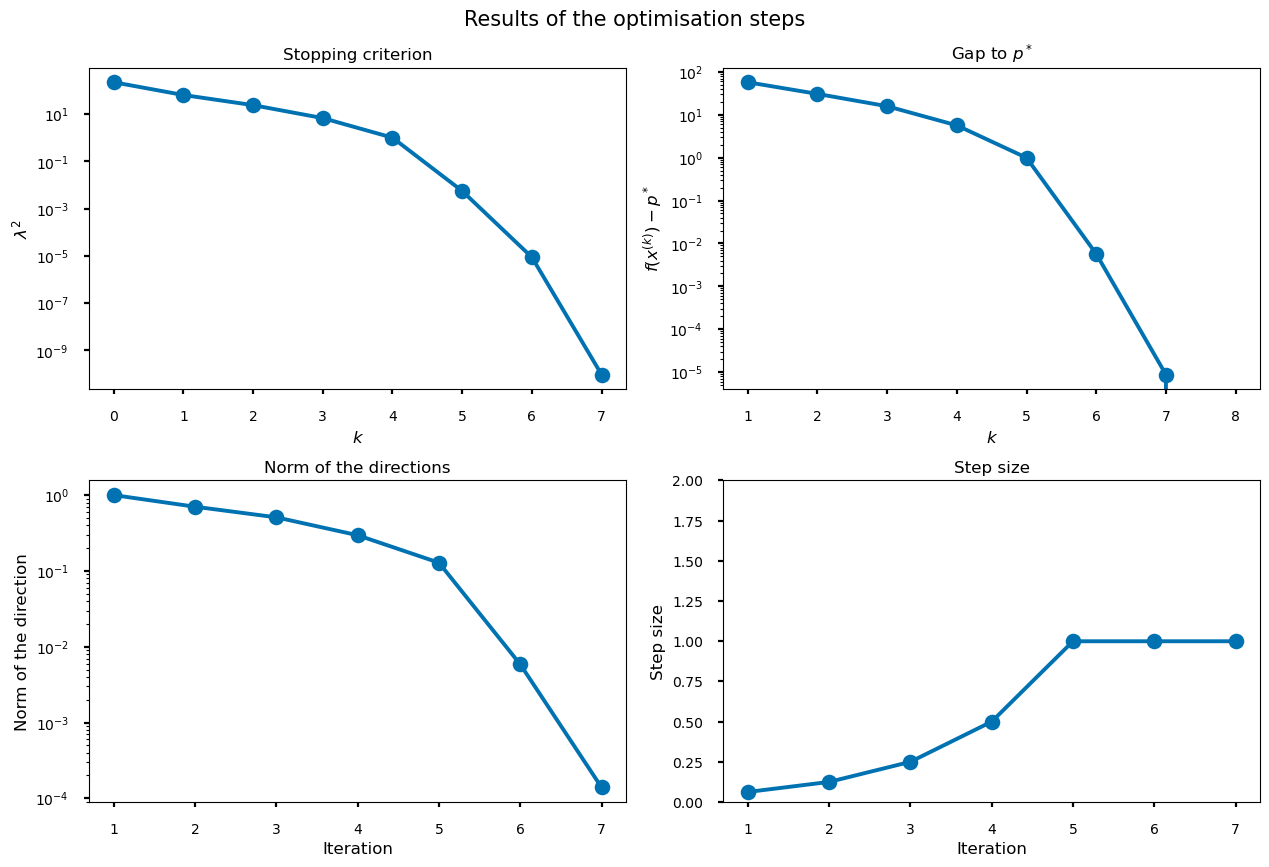
\includegraphics{outputs/example_output_centering.png}
\caption{Centering step output}
\end{figure}

Example output of a centering step for mu=10, t=100, alpha=0.1 and
beta=0.5

We clearly see the two parts of the method, as described in the course.

    \hypertarget{other-example}{%
\subsubsection{Other example}\label{other-example}}

On another note, I also used this method on a 2D function, given as an
example in the course, to plot the descent.

\begin{figure}
\centering
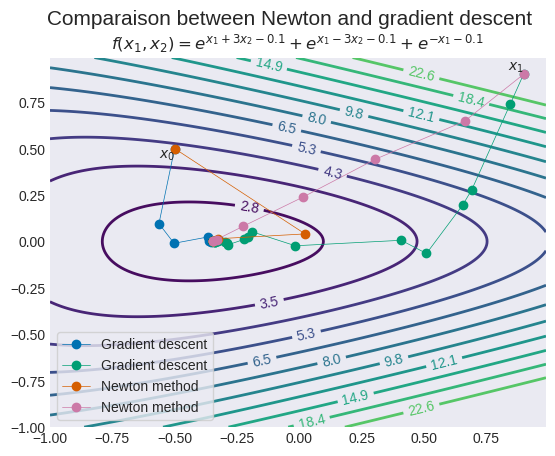
\includegraphics{outputs/comparaison_newton_gradient_4.png}
\caption{alt text}
\end{figure}

    \hypertarget{barrier-method}{%
\subsection{Barrier method}\label{barrier-method}}

This section presents results of the barrier method.

\begin{figure}
\centering
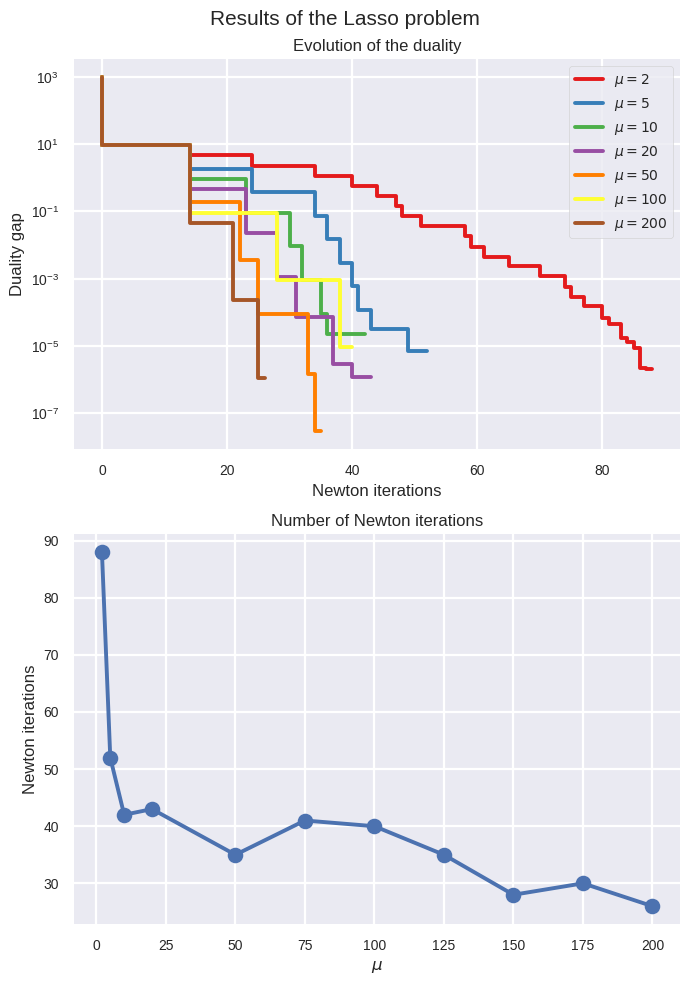
\includegraphics{outputs/lasso_pb_outputs.png}
\caption{Barrier method results}
\end{figure}


    % Add a bibliography block to the postdoc
    
    
    
\end{document}
